\chapter{State of the Art}\label{chapter:sota}
The chapter presents the state of the art (SotA) regarding technological approaches for GDPR compliance, with a particular focus and emphasis on those that utilise semantic web technologies.

Legal compliance as a field is quite broad due to the extent of laws which can be abstract (or universal) in their application or are intended to be enacted for a specific domain.
Achieving legal compliance is itself a large field of research, with technical approaches providing a special attraction in all domains due to the potential of automation and co-ordination with information management systems.
For the purposes of this thesis, the scope and focus is on technical approaches to assist the legal compliance process within the domain of GDPR compliance.

Before delving into approaches concerning GDPR, it is imperative to have an understanding of the field concerning technological approaches used in legal compliance. As all approaches for legal compliance share their motivation and aims, understanding their commonality and rationale enables placing the work associated with GDPR compliance within the broader scope of legal compliance.
It also provides investigation of avenues where existing approaches developed for other areas of legal compliance could be reused for GDPR, while providing the necessary background for understanding some of the decisions made by approaches concerning GDPR compliance in reusing existing technologies developed for legal compliance.

Surveys analysing approaches over a period of time provide a good overview of the use of technology in addressing legal compliance.
One such survey  analyses technological approaches for legal compliance within the 50 years of 1957-2007 \cite{otto_addressing_2007} to provide categorisation based on the representation of information and a set of Requirements Engineering Objectives (REO) an approach must follow to assist the legal compliance process.
While the survey paper in does not explicitly refer to linked data principles \cite{bizer_linked_2011}, some of the REO are fulfilled by utilising linked data and semantic web to provide an interoperable representation based in standards to define the required metadata regarding legislations.

Where legal compliance is closely tied to the functioning of an organisation, the requirements of compliance need to be Incorporated into the relevant activities (commonly called \textit{business processes}) within the organisation.
As the GDPR dictates the use of personal data and also requires organisations to adopt practices such as provision of rights, the study of compliance approaches from the perspective of business processes is also relevant in understanding the state of the art. 
For this, two key surveys provide the necessary overview of the relation between business processes and compliance. The first survey \cite{fellmann_state---art_2014} relates to the use of business processes within different phases of compliance, and provides the basis for categorising approaches as ex-ante (a-priori, ad-hoc) and ex-post (a-posteriori, post-hoc) depending on whether the compliance is relevant before the activity (in this case processing of personal data) has taken place or after. The second survey \cite{benyoucef_information_2015} analyses the approaches utilising business processes for compliance, and concludes that compliance approaches are basically limited to identifying relevant requirements from laws and regulations and ensuring that business processes comply with them, without much attention to compliance enactment.

`Legal Ontologies' is an umbrella term used to represent ontologies that represent information associated with the legal domain.
Key surveys in this domain categorise and analyse ontologies based on 
purposes \cite{leone_taking_2019,rodrigues_legal_2019}, 
access control \cite{kirrane_access_2016}, 
rights expression languages \cite{pellegrini_genealogy_2018}, 
privacy policy languages \cite{van_de_ven_qualitative_2016}, and
privacy requirements engineering \cite{gharib_ontologies_2016}.
Ontologies have been extensively used for formal representations of information, rules \cite{kirrane_scalable_2018}, rights \cite{pellegrini_genealogy_2018}, legislations \cite{leone_taking_2019}, business processes \cite{elgammal_formalizing_2016}, policies \cite{van_de_ven_qualitative_2016}, and requirements \cite{gharib_ontologies_2016}.
In areas of compliance, standardisation of representations for norms and requirements has seen efforts such as LegalRuleML \cite{palmirani_legalruleml_2011} which uses temporal and defeasible logic, and has been applied for compliance checking over business processes \cite{governatori_semantic_2016}. On similar lines, Compliance Management Ontology \cite{syed_abdullah_compliance_2012} proposes shared conceptualisation of business process management, culture management, obligations, programme, resources, risk management, and solutions.
There has also been a noted lack of guidelines regarding their reuse, particularly within the legal domain for compliance \cite{casanovas_legal_2017} where evaluation of developed ontologies is a challenge due to the requirement of specialists or legal experts being involved in the modelling stage \cite{rodrigues_legal_2019}.

The state of the art in technologies used for legal compliance thus presents encompassing representations for documents, requirements, rules, obligations, policies, and business processes associated with legal compliance. An adopter has a range of approaches to choose from based on existing approaches and formalisms, where the choice of approach is based on the stated requirements and goals as well as its role in the legal compliance process.

Given the motivation of this thesis in utilising semantic web technologies, and the research question exploring activities associated with personal data and processing for GDPR compliance - the state of the art is presented as an overview of approaches within the scope of these topics - with other approaches also presented to present the relevance of work developed within the domain.

The chapter is structured as follows: the first section (\autoref{sec:sota:methodology}) presents an overview of the methodology used to identify and analyse the state of the art. 
The second section (\autoref{sec:sota:gdpr-semweb}) presents approaches using semantic web technologies to address GDPR compliance, with the third section  (\autoref{sec:sota:gdpr-other}) presenting approaches addressing GDPR compliance using technologies other than semantic web.
The fourth section (\autoref{sec:sota:privacy-policies}) presents approaches regarding privacy policies in the context of GDPR which feature information relevant to the compliance process while not addressing compliance itself directly.
The fifth section (\autoref{sec:sota:consent}) presents approaches that concern representation of consent as required by GDPR.
The chapter concludes with an analysis of the SotA (\autoref{sec:sota:analysis}). It identifies gaps within the SotA and discusses the research opportunities to address them.

\section{Methodology}\label{sec:sota:methodology}

\subsubsection{Identification and classification of approaches}
The identification of approaches was carried out throughout the development of research presented in this thesis given the evolving nature of information about GDPR and legal opinions on its compliance.
Given the research question and motivation of this thesis, the scope of work considered as the state of the art was defined as \textit{approaches addressing GDPR compliance through technological solutions}, with a particular emphasis on the approach being published in an accessible manner.

Peer-reviewed publications were the primary source of knowledge regarding the approaches, identified using scholarly indexing services such as Google Scholar\footnote{\url{https://scholar.google.com/}}, IEEE Explore\footnote{\url{https://ieeexplore.ieee.org/}}, ACM Digital Library\footnote{\url{https://dl.acm.org/}}, Scopus\footnote{\url{https://www.scopus.com/}}, and DBLP\footnote{\url{https://dblp.uni-trier.de/}}.
In addition to these, information was also gathered through dissemination networks such as Twitter\footnote{\url{https://twitter.com/}} and mailing lists.
Searches using keywords such as \textit{GDPR}, \textit{GDPR Compliance}, and \textit{Consent} were used to identify relevant approaches in these sources and added to a reference manager (Zotero\footnote{\url{https://zotero.org/}}).
Authors and affiliations of identified publications were also used as keywords to find additional relevant resources.
In cases where the publication acknowledged a particular funding or project, an effort was made to identify its online website and access the list of publications. This also provided information about the project's aims and objectives, and its future goals and directions. 

Publications behind paywalls which could not be accessed either as a pre-print found elsewhere or by contacting the author with a request to access were not added to the state of the art and are not presented in this thesis. Requests for access to resources mentioned within a publication was also made where possible, with a resource considered `open' if published and `accessible' if it could be accessed. Commercial solutions of GDPR compliance are not considered to be within the state of the art given their closed nature and lack of knowledge regarding implementations.

Based on the approaches collected, they were categorised based on their relevance to the research question of this thesis.
Approaches addressing GDPR with a particular emphasis on utilising semantic web are presented in \autoref{sec:sota:gdpr-semweb} with the other approaches addressing GDPR compliance presented in \autoref{sec:sota:gdpr-other}.

\subsubsection{Criteria for Analysis}
Analysis of the state of the art is based on two surveys regarding
classification of approaches for legal compliance \cite{otto_addressing_2007} and phases of compliance \cite{fellmann_state---art_2014} that provide context and features to represent the analysis.
The research questions and objectives provide the basis for constructing a set of questions for the investigation of approaches within the state of the art.
The questions are stated below with an indication to the relevant research question and objective guiding this thesis:
\begin{enumerate}
    \item Which aspects of GDPR compliance does the approach target? ($RO1$, $RO2$)
    \item How does the approach represent information associated with GDPR and its compliance? ($RO3$)
    \item How does the approach link information with GDPR? ($RO3(a)$)
    \item How does the approach represent activities associated with processing of personal data and consent? ($RQ3(b)$)
    \item Does the approach provide indication of ex-ante and ex-post phases of activities for compliance? ($RO2$, $RO3$)
    \item How does the approach represent information associated with consent? ($RO3(c)$)
    \item How does the approach query information relevant to compliance? ($RO4$)
    \item How does the approach validate information relevant to compliance? ($RO5$)
    \item How does the approach evaluate GDPR compliance? ($RO5$)
\end{enumerate}

Based on these, the approaches within the SotA are analysed to identify if they: (i) represent clauses and concepts of GDPR, (ii) provide a data model of concepts such as an ontology, (iii) represent information for ex-ante compliance, (iv) represent information for ex-post compliance, (v) model process flows/activities, (vi) model consent information, (vii) evaluate GDPR compliance, (viii) specify requirements for compliance, and (ix) provide their resources in an open and accessible manner to enable its introspection.

These questions and criteria are used to assess the approaches with their analysis provided in \autoref{sec:sota:analysis} at the conclusion of this chapter.
The analyses is presented in sections associated with representation of GDPR, representation of activities, representation of consent, querying of information for compliance, and evaluation of GDPR compliance.

\section{Approaches for GDPR compliance utilising Semantic Web}\label{sec:sota:gdpr-semweb}

\subsubsection{SPECIAL}\label{sec:sota:SPECIAL}
SPECIAL\footnote{\url{https://www.specialprivacy.eu/}} (Scalable Policy-aware Linked Data Architecture For Privacy, Transparency and Compliance) is an European H2020 Project that aims to provide technical solutions for data protection requirements associated with use-cases involving big data. It features extensive use of semantic web technologies across a variety of compliance related tasks such as recording provenance logs of data processing \cite{kirrane_scalable_2018}, providing visual interfaces for consent \cite{drozd_consent_2019,gritzalis_i_2019}, compliance checking of processing activities based on given consent \cite{westphal_spirit_2018,vos_odrl_2019,fernandez_user_2019}, and efforts towards standardisation of related vocabularies\footnote{The SPECIAL project was the primary driving force behind the creation of the W3C Data Privacy Vocabularies and Controls Community Group (DPVCG), of which the author was an active participating member. Information about this has been listed in \autoref{sec:intro:dpvcg}. The Data Privacy Vocabulary (DPV), produced by the DPVCG, has also been documented as a deliverable of the project in D6.5 \cite{pandit_d6.5_2019}.} \cite{bonatti_data_2018,pandit_creating_2019}.
Collaborations between SPECIAL and other projects have produced related work, such as an approach for compliance checking using ODRL \cite{agarwal_legislative_2018,vos_odrl_2019}, and the application of SPECIAL's framework in a Smart City use-case \cite{fernandez_user_2019}.
Information about the methodologies used, developed technologies, and their evaluations is accessible through peer-reviewed publications and public deliverables\footnote{\url{https://www.specialprivacy.eu/publications/public-deliverables}}.

SPECIAL uses a distributed ledger to store the processing logs for data processing activities, which can be evaluated for compliance against given consent in ex-ante and ex-post phases. The logs are stored using the  Policy Log vocabulary\cite{bonatti_special_2018-1} with the data processing activities represented by Usage vocabulary \cite{bonatti_special_2018-2}. Compliance evaluation is performed by using a custom reasoning algorithm \cite{bonatti_fast_2018,bonatti_richer_2019} in a semantic reasoner. The consent is provided in a visual and interactive form to the user using the web browser \cite{drozd_consent_2019,gritzalis_i_2019}. The project has been successfully applied to use-cases provided by its commercial partners\footnote{See D1.5 \cite{bonatti_d1.5_2018} and D1.6 \cite{schlehahn_d1.6_2018} for information on use-cases.} as well as in an external use-case related to use of IoT in Smart Cities \cite{fernandez_user_2019}. The Figure. \ref{fig:SPECIAL-architecture1} presents an overview of the SPECIAL architecture along with its components and utilised technologies.
\begin{figure}[htbp]
    \centering
    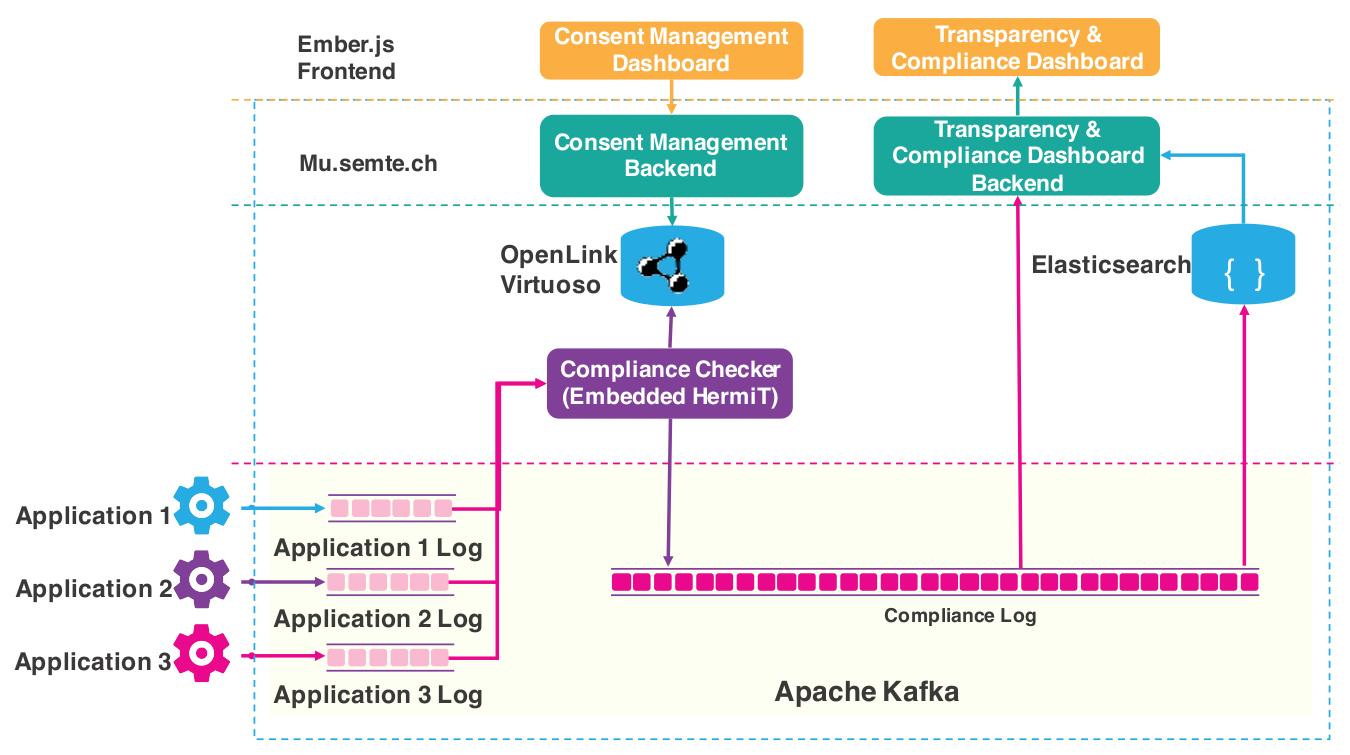
\includegraphics[width=\linewidth]{img/SPECIAL_architecture1.png}
    \caption{Overview of SPECIAL Architecture \cite{kirrane_scalable_2018}}
    \label{fig:SPECIAL-architecture1}
\end{figure}

The ontology developed to represent data processing activities is called `Usage Policy' \cite{bonatti_special_2018-2} is described in more detail in D2.5 \cite{bonatti_d2.5_2018}. The `base policy' denotes a ontology design pattern of OWL2 expressions to denote an intersection of personal data categories, processing operations, purposes, recipients, and storage. Policies can then be combined using OWL2 unions over multiple base policies with differing expressions. SPECIAL provides additional vocabularies for purposes, personal data categories, processing operations, and recipients for using with the Usage Policy based on its use-cases. The general form of a base policy is:
\begin{listing}[htbp]
\begin{minted}{scheme}
ObjectIntersectionOf(
    ObjectSomeValuesFrom(spl:hasData SomeDataCategory)
    ObjectSomeValuesFrom(spl:hasProcessing SomeProcessing)
    ObjectSomeValuesFrom(spl:hasPurpose SomePurpose)
    ObjectSomeValuesFrom(spl:hasRecipient SomeRecipient)
    ObjectSomeValuesFrom(spl:hasStorage SomeStorage)
)
\end{minted}
\end{listing}
The storage expression is itself a policy comprising of OWL2 expressions specifying the storage location, duration, and interval. The general form of a storage policy is:
\begin{listing}[htbp]
\begin{minted}{scheme}
ObjectIntersectionOf(
    ObjectSomeValuesFrom(spl:hasLocation SomeLocation)
    ObjectSomeValuesFrom(spl:hasDuration SomeDuration)
    DataSomeValuesFrom(spl:durationInDays Interval)
)
\end{minted}
\end{listing}

For a given policy $P_c$ representing activities permitted by given consent and policy $P_s$ representing processing activity, compliance is evaluated by checking whether $P_c$ complies with $P_s$ - which in OWL2 is checked using a semantic reasoner to evaluate $P_c \subseteq P_s$. In SPECIAL's implementation, this is performed by using an algorithm \cite{bonatti_fast_2018,bonatti_richer_2019} in a custom semantic reasoner optimised for speed by only performing those operations associated with checking for compliance between policies.
An extension of the Usage Policy for representing additional requirements of the GDPR was discussed in the deliverable D2.6 \cite{bonatti_d2.6_2018}.

The activity is recorded in a log entry using the Policy Log vocabulary \cite{bonatti_special_2018-1}, represented in Figure. \ref{fig:SPECIAL-policy-log-vocabulary} by the concept \texttt{LogEntry}, and is evaluated for compliance by using the reasoner in both ex-ante and ex-post phase. 
\begin{figure}[htbp]
    \centering
    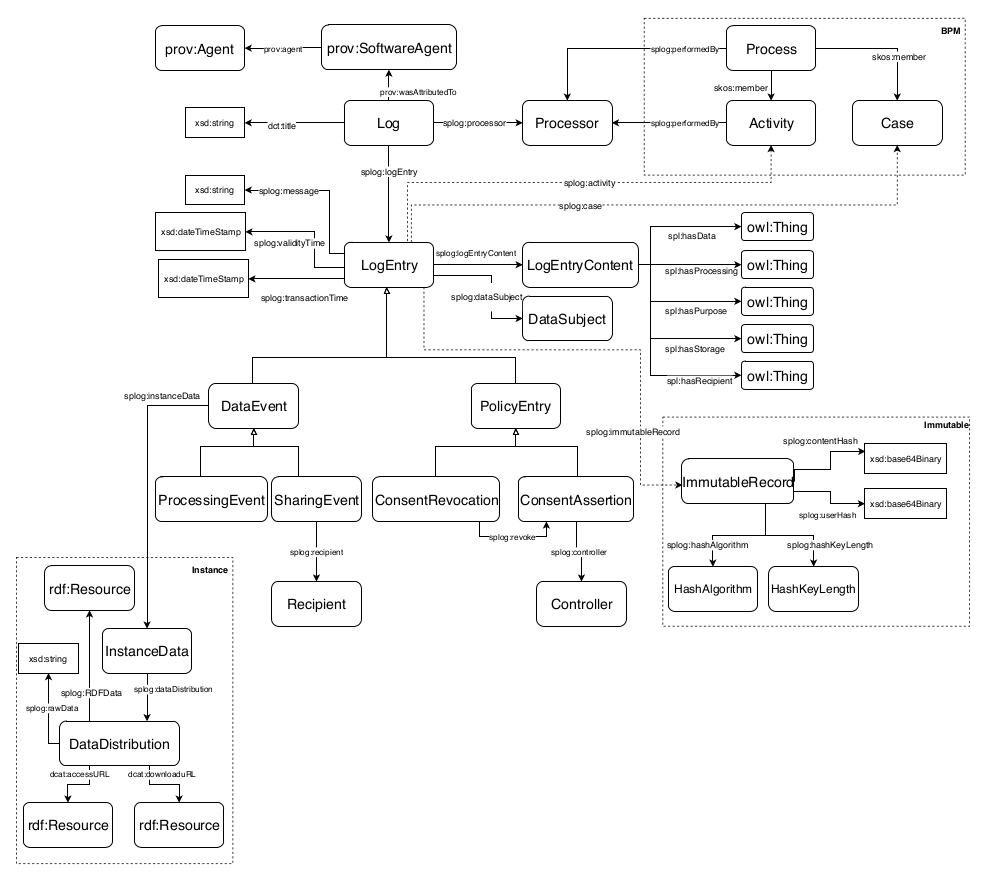
\includegraphics[width=0.8\linewidth]{img/SPECIAL_logvocabulary.png}
    \caption{Overview of SPECIAL Policy Log Vocabulary \cite{bonatti_special_2018-1}}
    \label{fig:SPECIAL-policy-log-vocabulary}
\end{figure}

The Policy Log vocabulary, described in D2.7 \cite{kirrane_d2.7_2018}, reuses existing vocabularies of DCAT and PROV-O \cite{lebo_prov-o_2013}, and is used to record an immutable documentation of compliant activities and their legal basis in consent. Each log entry contains information about the agent that created the log (\texttt{prov:SoftwareAgent} and \texttt{Log}), a link to the data subject, and information about the processing through the concept \texttt{LogEntryContent} which contains information represented using concepts from the base policy.
Information about consent is recorded through \texttt{PolicyEntry} and consists of consent assertion (given consent) and consent revocation (withdrawn consent).

The methodologies associated with the vocabularies produced by the SPECIAL project are based on the utilisation of metadata in the compliance process \cite{wenning_compliance_2018}. The creation of policy vocabularies from use-cases is described through the public deliverable D1.5 \cite{bonatti_d1.5_2018}, with that of the log vocabulary provided in D3.2 \cite{kirrane_d2.7_2018}. The vocabularies created by the project are documented and publicly accessible online.

\subsubsection{SERAMIS}
SPECIAL's work has also produced ODRL models for deontic representations of GDPR requirements through collaborations with other projects. The first of this is based on work with the Austrian SERAMIS\footnote{\url{https://cordis.europa.eu/project/rcn/189040/factsheet/en}} (Sensor-Enabled Real-World Awareness for Management Information Systems) project, which produced a web-based tool called PriWUcy for evaluating compliance assessments of GDPR articles \cite{agarwal_d5.5_2017,agarwal_legislative_2018}.
The tool uses a model of the legislation created by parsing the legislation text and representing the obligations using ODRL. A set of preliminary assessment questions provides the inputs over which the model is applied to identify actions and obligations to be fulfilled as part of the assessment. The ODRL model, depicted in Figure. \ref{fig:SPECIAL-ODRL}, is extended to represent additional granularity of constraints of - Feature, Discretional, and Dispensation. The ODRL policies are associated with the text of the GDPR they represent through classes representing chapters, articles, and paragraphs within the text of the GDPR. The approach relies on identifying and representing assets, parties, actions, duties, and constraints using the developed ODRL model.
\begin{figure}[htbp]
    \centering
    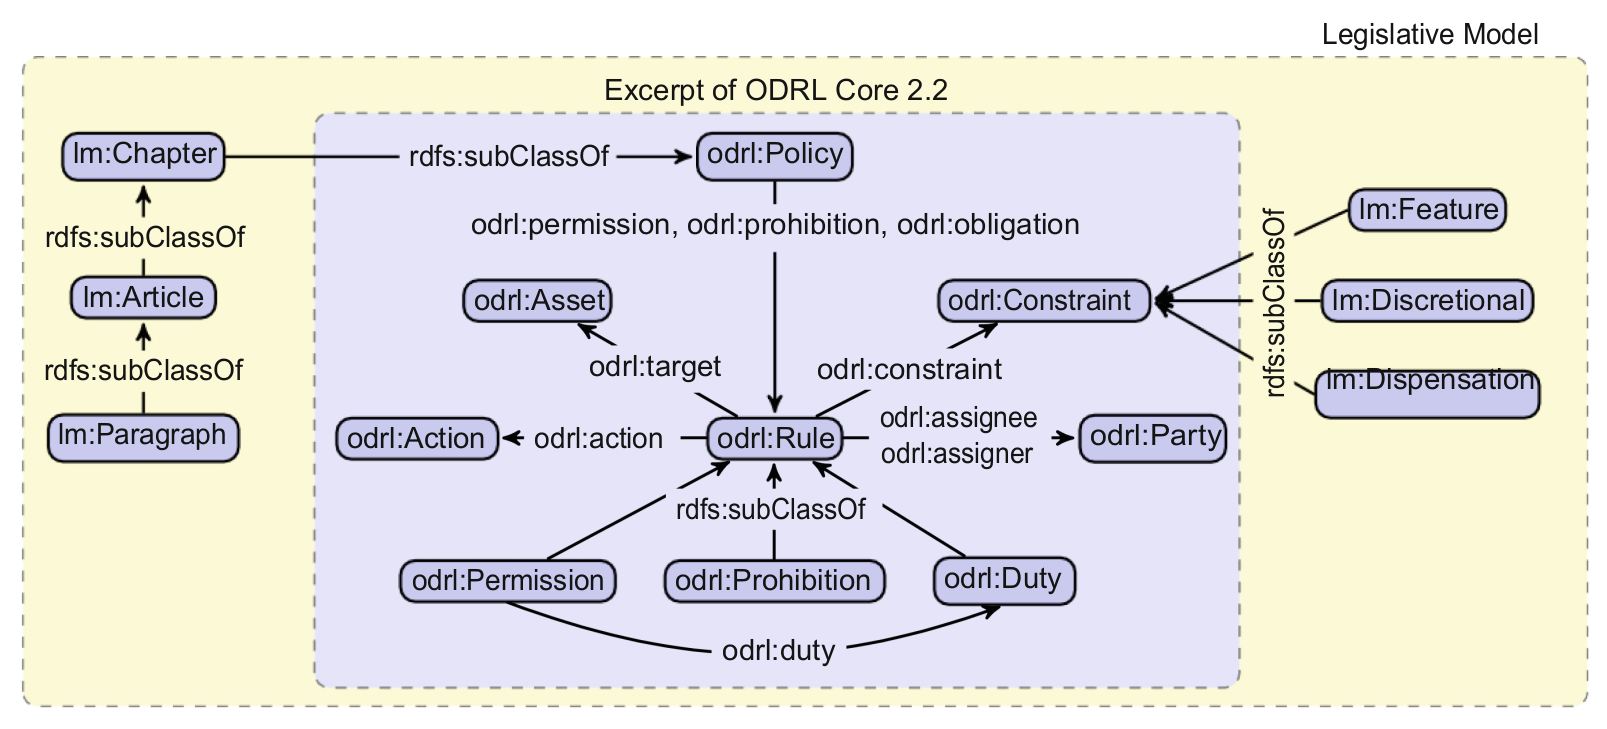
\includegraphics[width=\linewidth]{img/SPECIAL_ODRL.png}
    \caption{Extension of ODRL for representing GDPR obligations \cite{agarwal_legislative_2018}}
    \label{fig:SPECIAL-ODRL}
\end{figure}

\subsubsection{Vos et al.}
The ODRL profile was further developed for modelling regulatory obligations and business policies based on GDPR towards compliance checking and providing explanations of the reasoning process \cite{vos_odrl_2019}. Additional classes and properties added include those relevant for specifying the legal basis, purpose, location, and safeguards associated with processing. Policies representing articles in the GDPR are checked against permissions by activities to perform a data processing operation. For example, the following listing shows a request to transfer personal data to a third country based on consent, which would be checked against the corresponding policy representing Article 46 of the GDPR. 
\begin{listing}[htbp]
\begin{minted}{turtle}
<http://example.com/policy:bp-transfer> a orcp:Set ;
    odrl:profile <http://example.com/odrl:profile:regulatory-compliance> ;
    orcp:permission
    [ odrl:action orcp:Transfer ;
        orcp:data orcp:PersonalData ;
        orcp:responsibleParty orcp:Controller ;
        orcp:organisationType orcp:InternationalOrganisation ;
        orcp:sender <http://example.com/CompanyA_Ireland> ;
        orcp:recipient <http://example.com/CompanyA_US> ;
        orcp:recipientLocation orcp:ThirdCountry ;
        orcp:purpose orcp:PersonalRecommendations ;
        orcp:legalBasis orcp:Consent ;
        odrl:dataSubjectProvisions orcp:EnforceableDataSubjectRights ;
        odrl:dataSubjectProvisions orcp:LegalRemediesForDataSubjects
    ] .
\end{minted}
\end{listing}
Compliance is checked by converting the ODRL policies into InstAL, a domain-specific language for writing models based on events and states, which translates to Answer Set Programming (ASP) and is evaluated using a Answer Set Solver\footnote{CLINGO \url{https://potassco.org/clingo/}}. When a policy is found to be non-compliant, explanations are generated based on `fluents' - facts that are true if present and false if absent - through a reasoning process. The implementation is publicly accessible through a hosted repository\footnote{\url{https://github.com/instsuite/instsuite.github.io/blob/master/gdpr.ial}}. 
% An example of this is as follows:
% \begin{lstlisting}
% # fluents capturing justifications
% type Article;
% fluent permission(Subject,Article);
% fluent prohibition(Subject,Article);
% noninertial fluent supports(Subject,Article,Predicate,Object);
% noninertial fluent lacks(Subject,Article,Predicate,Object);

% # if enforceable data subject rights are defined, the term is true
% article46_body_term2(Process) when
%     triple(Process,dataSubjectProvisions,enforceableDataSubjectRights);
% supports(Process,article46,dataSubjectProvisions,
%         enforceableDataSubjectRights) when
%     article46_body_term2(Process),
%     triple(Process,dataSubjectProvisions,enforceableDataSubjectRights);

% # otherwise the description lacks data, and non-inertial fluents are applied
% lacks(Process,article46,dataSubjectProvisions,
%         enforceableDataSubjectRights) when
%     applies(Process,article46),
%     not supports(Process,article46,dataSubjectPro
% \end{lstlisting}

\subsubsection{CitySPIN}
The second work is based on applying SPECIAL's GDPR compliance framework to the Austrian CitySPIN\footnote{\url{http://cityspin.net/}} (Cyber-Physical Social Systems for City-wide Infrastructures) project \cite{fernandez_user_2019}, which utilises linked data platforms to ingest data from multiple sources in a smart city scenario, and utilises it for data processing pipelines and analytics. An important component of the project is the management of consent which utilises SPECIAL's policies \cite{bonatti_special_2018-1,bonatti_special_2018-2} and compliance framework \cite{kirrane_scalable_2018}.
\autoref{fig:SPECIAL-CitySPIN} presents an overview of CitySPIN and its relation with the SPECIAL vocabularies. The auxiliary vocabularies provided by SPECIAL for purpose and data categories (SPECIAL-MCM in figure) were extended for use-cases associated with CitySPIN (CPSS Core vocabulary and UC vocabulary in figure).
The figure uses white blocks indicating concepts from SPECIAL's vocabularies and the others indicating additional concepts defined by CitySPIN.
The defined policies are checked in the ex-ante and ex-post phase using the SPECIAL compliance checking algorithm \cite{bonatti_fast_2018,bonatti_richer_2019}, with a prototype implementation demonstrating ex-ante compliance checking in ad-hoc widgets sharing personal data \cite{fernandez_privacy-aware_2019}. Details about the project and its implementation are available through its public deliverables D6.1 \cite{noauthor_d6.1_2018} and D6.3 \cite{noauthor_d6.3_2019}.
\begin{figure}[htbp]
    \centering
    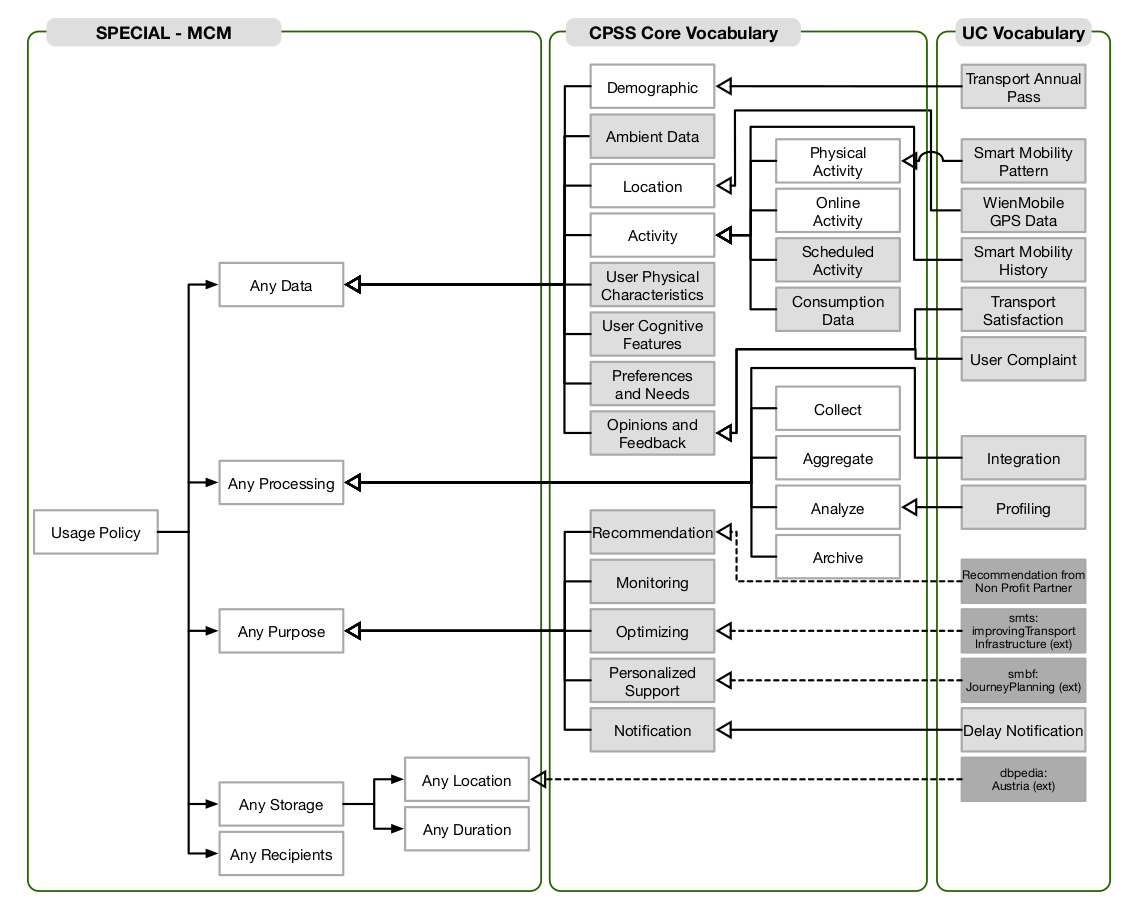
\includegraphics[width=0.8\linewidth]{img/SPECIAL_CitySPIN.png}
    \caption{CitySPIN's extension of SPECIAL vocabularies \cite{fernandez_user_2019}}
    \label{fig:SPECIAL-CitySPIN}
\end{figure}

The use-cases utilised within the SPECIAL project and a discussion of their legal requirements can be found in the deliverables D1.5 \cite{bonatti_d1.5_2018} and D1.6 \cite{schlehahn_d1.6_2018}. A dashboard representing information of processing activities and consent was created to represent the logged information \cite{raschke_designing_2017}, whose usability and testing are described in deliverables D4.3 \cite{raschke_d4.3_2019} and D4.4 \cite{milosevic_d4.4_2019}. Another visual interface for interactive consent was also developed based on presenting the components of a usage policy to the individual in an interactive format \cite{gritzalis_i_2019}. The interface provides visual representations of associations between purposes, processing, data categories, recipients, and storage which allows the individual to explore and choose their consent. It also offers visual paradigms such for representation of information as tabs, breadcrumbs, hierarchies, and graphs for visualisation and exploration of information. 

\subsubsection{MIREL}\label{sec:sota:MIREL}
MIREL\footnote{\url{www.mirelproject.eu/}} (Mining and Reasoning with Legal Texts) is an European H2020 Project that aims to create a framework for interpretation of legal texts into formal representations for querying norms, checking legal compliance, and decision support. The project uses semantic web to provide normative requirements \cite{gandon_normative_2017}, provide natural language processing over legal texts \cite{teruel_legal_2018}, and creating ontologies based on GDPR \cite{monica_legal_2018} for legal compliance \cite{palmirani_pronto_2018-1} and reasoning \cite{palmirani_pronto_2018}. The project also involves creation of icons for data protection based on the developed ontologies \cite{arianna_dapis_2019}.
Information about the project is available through peer-reviewed publications and public deliverables\footnote{\url{http://www.mirelproject.eu/publications.php}}.
Details about the project and its developed resources, namely PrOnto, have  been described in publications, but are not open or publicly accessible at the time of writing this thesis.

The developed ontology is termed PrOnto (Privacy Ontology) \cite{monica_legal_2018}, and provides concepts within the GDPR associated with data types and documents, agents and roles, processing purposes, legal bases, processing operations, and deontic operations for modelling rights and duties. It reuses existing vocabularies \cite{palmirani_pronto_2018} and has been applied within the Cloud4EU project\footnote{\url{http://www.agid.gov.it/cloudforeurope}} for legal compliance checking of eGovernment systems as well as the DAPRECO project.
PrOnto was developed using the MeLOn (Methodology for building Legal Ontologies) developed in the MIREL project \cite{palmirani_pronto_2018,palmirani_pronto_2018-1,monica_modelling_2018}.

PrOnto consists of modules representing (i) documents and data (depicted in \autoref{fig:PrOnto-data}), (ii) actors and roles, (iii) processing and workflow, (iv) legal rules and deontic formula, (v) purposes and legal bases. It also includes modules for risk analysis and measures, which it utilises to represent risk management processes such as DPIA as workflows \cite{palmirani_pronto_2018}. Reasoning is utilised based on the deontic operators within the ontology, and violations are connected with the violated obligations thereby providing traceability towards the steps that created the violation. LegalRuleML is extended and used to represent the obligations and enable creation and rules for compliance.
\begin{figure}[htbp]
    \centering
    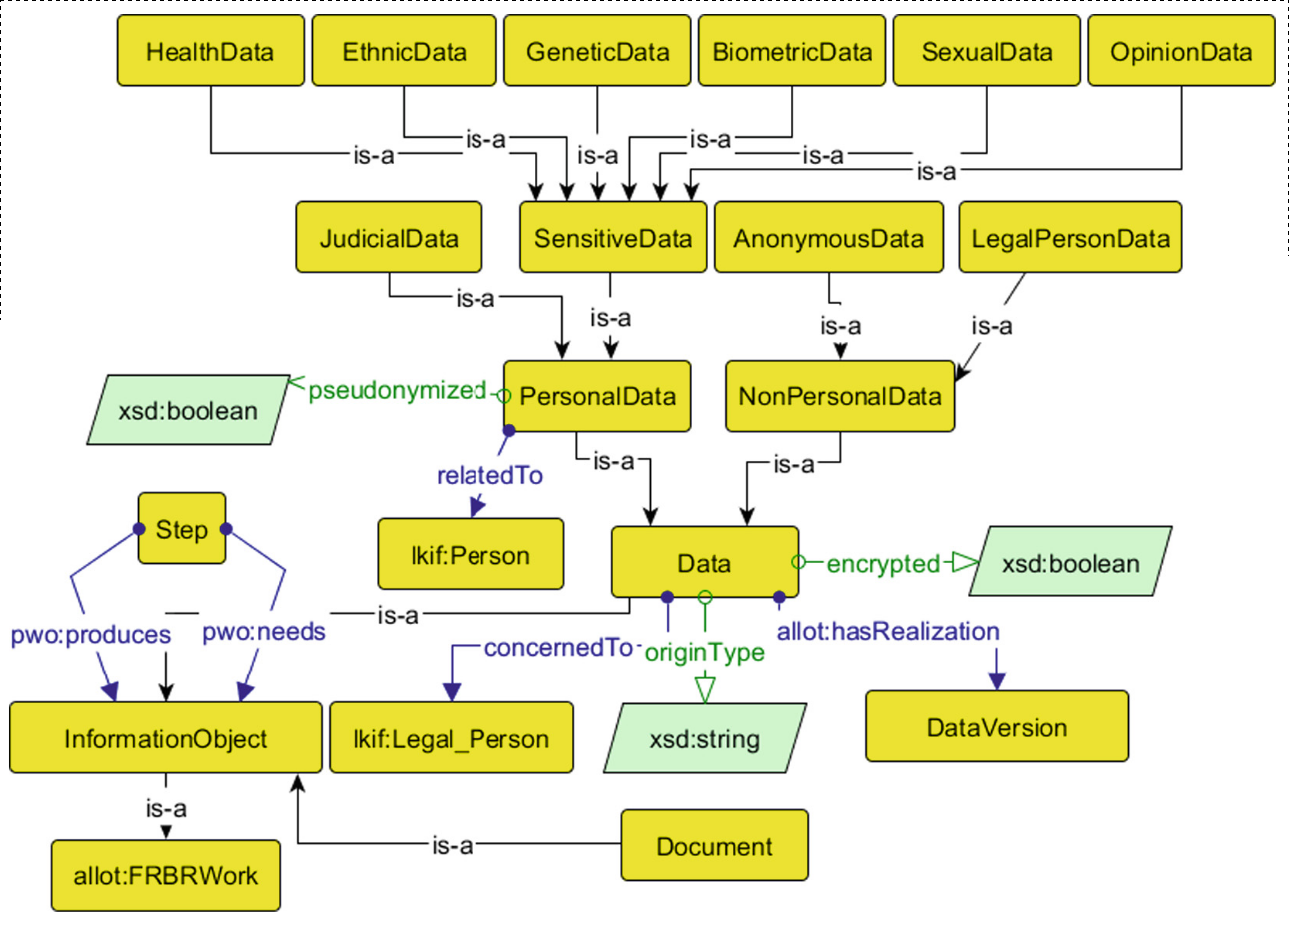
\includegraphics[width=0.8\linewidth]{img/PrOnto_data.png}
    \caption{Data Categories represented in PrOnto \cite{palmirani_pronto_2018}}
    \label{fig:PrOnto-data}
\end{figure}

A proof-of-concept application for detecting violations of the GDPR \cite{monica_modelling_2018} utilised PrOnto to model the legal concepts, along with Akoma Ntoso to model the legal text, LegalRuleML to model norms, and Regorous to apply LegalRuleML rules over BPMN and generate a report. The application utilises a web editor for modelling legal rules in connection with the legal text and ontology.

\subsubsection{DAPRECO}\label{sec:sota:DAPRECO}
DAPRECO\footnote{\url{https://www.fnr.lu/projects/data-protection-regulation-compliance/}} (Data Protection Regulation Compliance) is an Luxembourgian project relating to the creation of a knowledge base for formal compliance with the terms and provisions of the GDPR. It aims to provide formalisms in deontic logic and natural language semantics for handling legal norms in written language. The project has researched correlation of standards with laws \cite{bartolini_towards_2016}, creation of an ontology to model concepts in the GDPR \cite{otake_using_2017}, modelling the norms of the GDPR using logic formalisms \cite{bartolini_legal_2018}, and annotating BPMN for GDPR compliance \cite{bartolini_enhancing_2019}.
The project involves collaborations with the MIREL project, particularly in the creation and utilisation of PrOnto for addressing GDPR \cite{monica_legal_2018,palmirani_pronto_2018,palmirani_pronto_2018-1,bartolini_enhancing_2019}. In turn, DAPRECO provides a practical application of PrOnto as an use-case for legal compliance over business activities \cite{bartolini_enhancing_2019,bartolini_agile_2019}.

While PrOnto represents a more mature and progressive deliverable of the project's ontology for GDPR, the earlier ontology - referred to as data protection ontology \cite{otake_using_2017} - is relevant for its modelling of the concepts and norms based on an draft of the GDPR. This ontology uses OWL2 to model the concepts of the GDPR and was specified to be a work in progress in its publication\footnote{It can be assumed the ontology is no longer being used or developed and was utilised in the development of PrOnto based on subsequent publications of the project \cite{bartolini_legal_2018,bartolini_enhancing_2019}.}.
Its methodology consists of using the structure provided by the Handbook on European Data Protection Law\footnote{2014 edition \url{https://publications.europa.eu/en/publication-detail/-/publication/eee277d3-d26f-4a18-825b-8e1fd80d2f0d/language-en}}, and consists of concepts associated with - data protection principles, rules of data processing constituting duties of data controller, and data subject's rights.
The ontology reuses concepts from LKIF Core \cite{hoekstra_lkif_2007} to represent rights, rules, legal and natural persons. It establishes relations such as \textit{hasObligation} between a \textit{Controller} and a \textit{LegalObligation} concept, and \textit{consentGrantedBy} between \textit{Consent} and \textit{DataSubject} - representing the relations derived from GDPR.
The ontology was evaluated using the the OOPS! tool \cite{poveda-villalon_oops!_2014}, and was documented using the LODE \cite{peroni_tools_2013}. The ontology can be accessed publicly\footnote{Link from \cite{otake_using_2017} \url{https://github.com/guerret/lu.uni.eclipse.bpmn2}} with documentation provided using LODE ontology documentation tool \cite{peroni_tools_2013}.
The Competency Questions (CQ) representing functional requirements for the ontology were used in its evaluation through SPARQL queries, and are follows:
\begin{enumerate}
    \item What are the obligations of a data controller?
    \item What are the functions of a data processor?
    \item What are the rights of the data subject?
    \item How do the rights of the data subject relate to the obligations of the data controller and the functions of the processor?
    \item How can a data subject interact and/or enforce their rights against a data controller?
    \item What are the possible fines and sanctions issued in response to violations by data controllers?
    \item Who supervises a data controller?
\end{enumerate}

Subsequent applications of PrOnto in the project utilises Reified Input/Output logic (RIO) \cite{robaldo_reified_2017} - a formalism for normative reasoning based on reification applied to natural language semantics. The rules are expressed using LegalRuleML and are associated with activities using BPMN. This is utilised to allocate tasks related to data protection to stakeholders, and to track compliance across different phases of a software development life-cycle.
The project uses these to create a knowledge base \cite{bartolini_agile_2019} with feedback from stakeholders by providing a human-readable version of RIO logic rules utilised to model the GDPR. 
The project also researchers automating the comparison of GDPR with the ISO by extracting RIO rules from their texts and analysing them for comparisons.
The resulting knowledge base is used in collaboration with the MIREL project to provide semantic extraction and annotation over ECHR (European Court of Human Rights) judgements \cite{cardellino_legal_2017}, as described in MIREL's deliverables D2.4 \cite{robaldo_livio_d2.4_2017}.

\subsubsection{BPR4GDPR}\label{sec:sota:BPR4GDPR}
BPR4GDPR\footnote{\url{http://www.bpr4gdpr.eu/}} (Business Process Re-engineering and functional toolkit for GDPR compliance) is an European H2020 project that aims to provide a a reference compliance framework for the GDPR. The framework is stated to provide specification of sophisticated security and privacy policies, modelling technologies and tools for the incorporation of provisions in process models and the resulting executable processes, and means for automating verification and alignment.
This is planned to be achieved using a set of mechanisms for automating the respective procedures and resulting in processes that are compliant by design.
The project intends to implement the concept of Compliance-as-a-Service (CaaS) by providing a set of tools that fit the needs of various organisations being subject to GDPR compliance.
Information about the project is available through peer-reviewed publications and project deliverables\footnote{\url{http://www.bpr4gdpr.eu/results/deliverables/}}.

The project uses an ontology to represent the information model utilised in its approach, as depicted in \autoref{fig:BPR4GDPR-model} \cite{lioudakis_d3.1_2019}. The ontology consists of concepts and relationships regarding data types, roles, operations, and organisation types amongst other contextual concepts.
The ontology is serialised using OWL2, and contains `default instances' representing a ready to use set of instances based on its use-cases, which are described in detail in deliverable D3.1 \cite{lioudakis_d3.1_2019}. 
\begin{figure}[htbp]
    \centering
    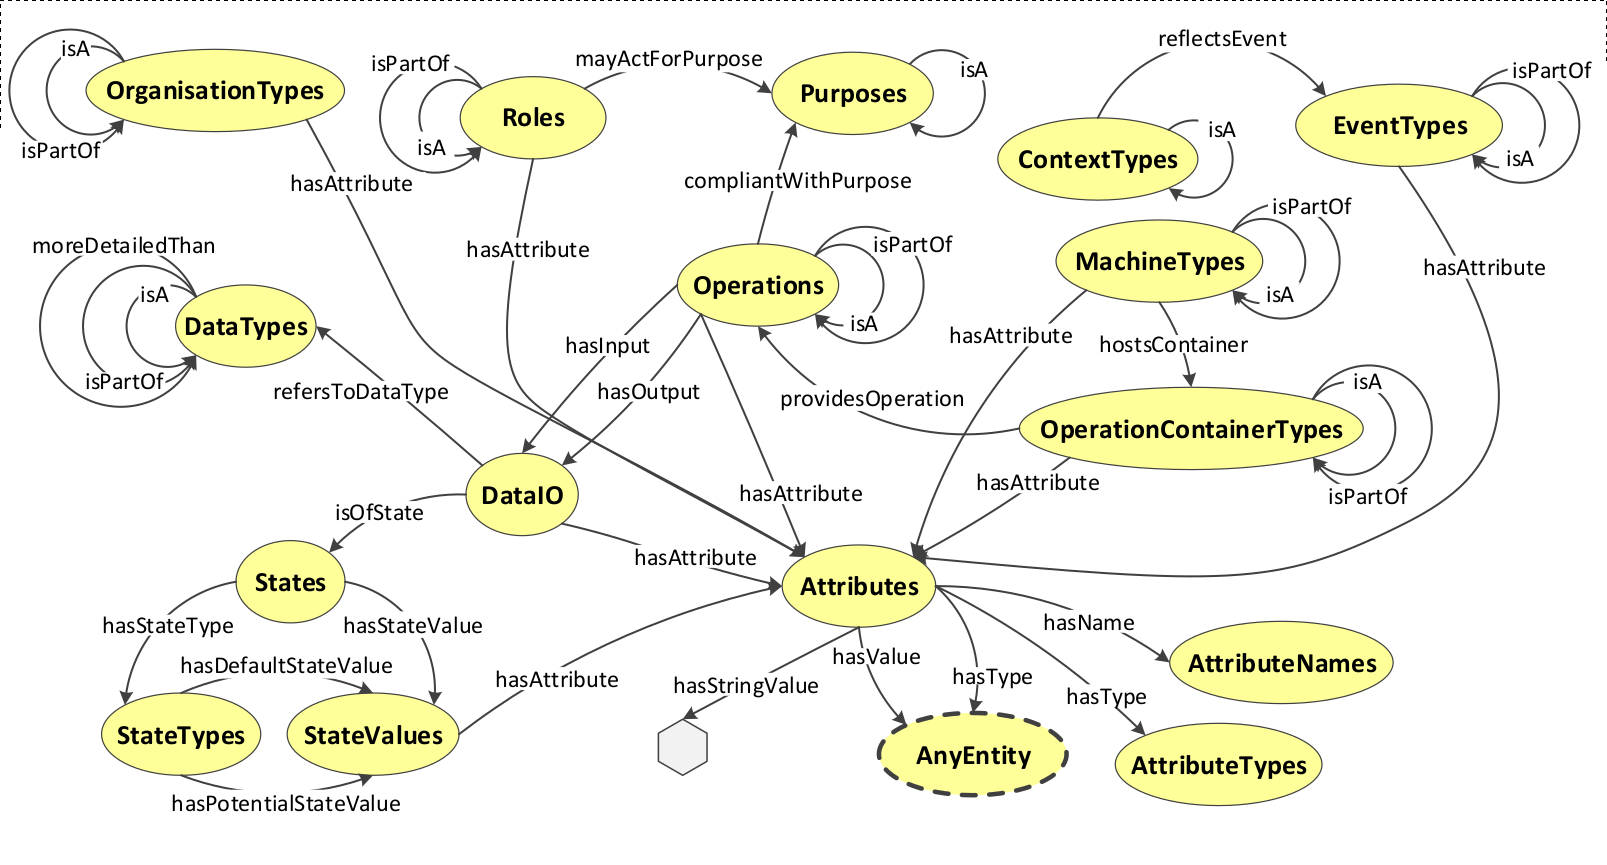
\includegraphics[width=0.8\linewidth]{img/BPR4GDPR_model.png}
    \caption{Information Model Ontology in BPR4GDPR \cite{lioudakis_d3.1_2019}}
    \label{fig:BPR4GDPR-model}
\end{figure}

The compliance assessment is performed using the compliance meta-model ontology, as depicted in \autoref{fig:BPR4GDPR-compliance}, and described in detail in deliverable D2.3 \cite{dellas_d2.3_2019}. The compliance ontology is used to dictate and evaluate processes by considering them as workflows where actions or operations are connected to each other in terms of dependencies and data flows, are performed by an actor, and include assets or artefacts.
\begin{figure}[htbp]
    \centering
    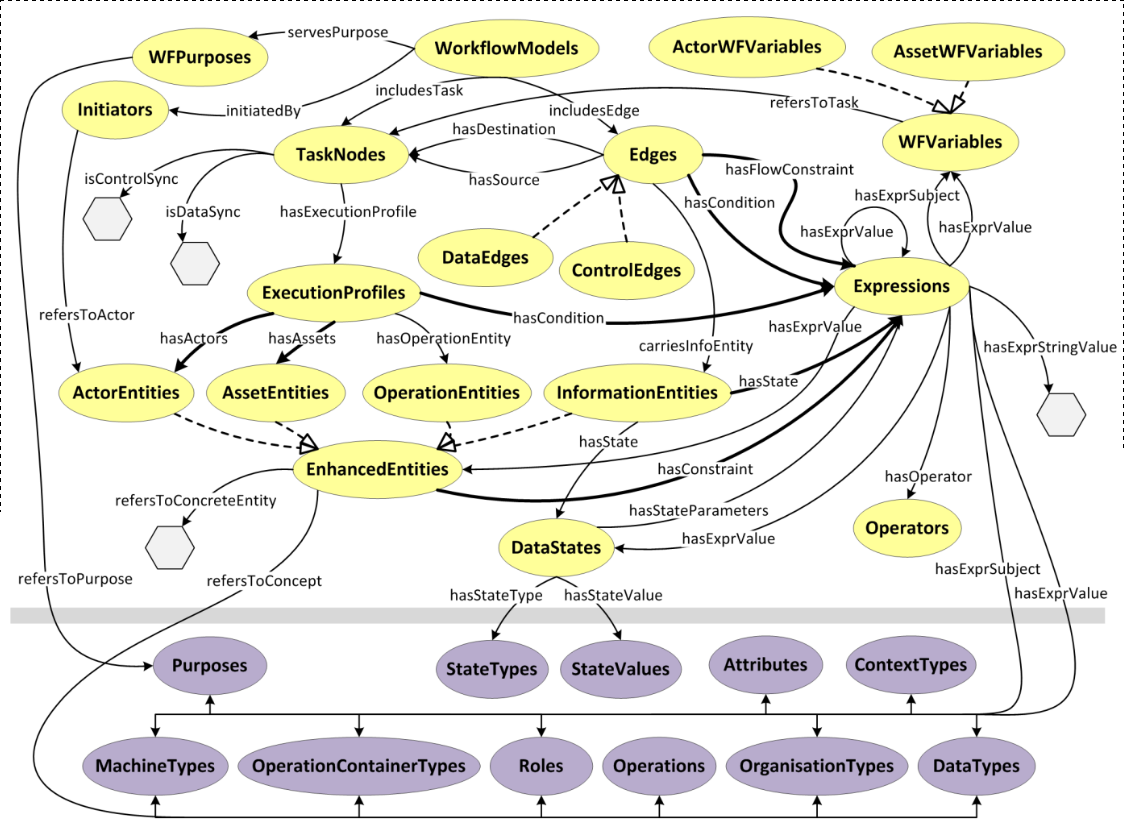
\includegraphics[width=0.8\linewidth]{img/BPR4GDPR_compliance.png}
    \caption{Compliance meta-model ontology in BPR4GDPR \cite{dellas_d2.3_2019}}
    \label{fig:BPR4GDPR-compliance}
\end{figure}

Process mining is performed on the knowledge extracted from the event logs of information systems to discover, monitor and improve processes not assumed or modelled prior to the evaluation. This is then utilised to create a process monitoring architecture, which contains the four sub-components of functionality
associated with pre-processing, conformance checking, rules, and model repair.
The approach intends to `repair' process models by analysing failed conformance checks, converted rules, and results of conformance checking to identify parts of the process model not compliant with the rules. 

The public deliverable D3.1 \cite{lioudakis_d3.1_2019} defines rules derived from the GDPR which represent the minimal set of configurations of the BPR4GDPR architecture before it is adapted to a particular use-case, i.e. its default configuration. These rules are intended to act as constraints in the conformance checking described above and used to repair the processes by identifying components that need to be changed to satisfy the rule.

\subsubsection{Elluri et al.}\label{sec:sota:Elluri}
Elluri et al. \cite{elluri_knowledge_2018, elluri_integrated_2018} present an ontology of rules and obligations for cloud data providers and consumers based on the GDPR and for Payment Card Industry Data Security Standard (PCI DSS). The ontology for GDPR \cite{elluri_knowledge_2018} is comprised of concepts for components - `Consumers and Providers', `Fines and Enforcement', `Breach \& Notification', `Data Protection Officer', and `Data Subject'. This is combined with the ontology developed for PCI DSS and Clous Security Alliance (CSA) to provide a comprehensive combined ontology for addressing their combined legal requirements and obligations \cite{elluri_integrated_2018}. The resulting ontology, depicted in \autoref{fig:Elluri-ontology}, consists of concepts and relationships associated with stakeholders, obligations for providers and consumers, and security requirements. 
\begin{figure}[htbp]
    \centering
    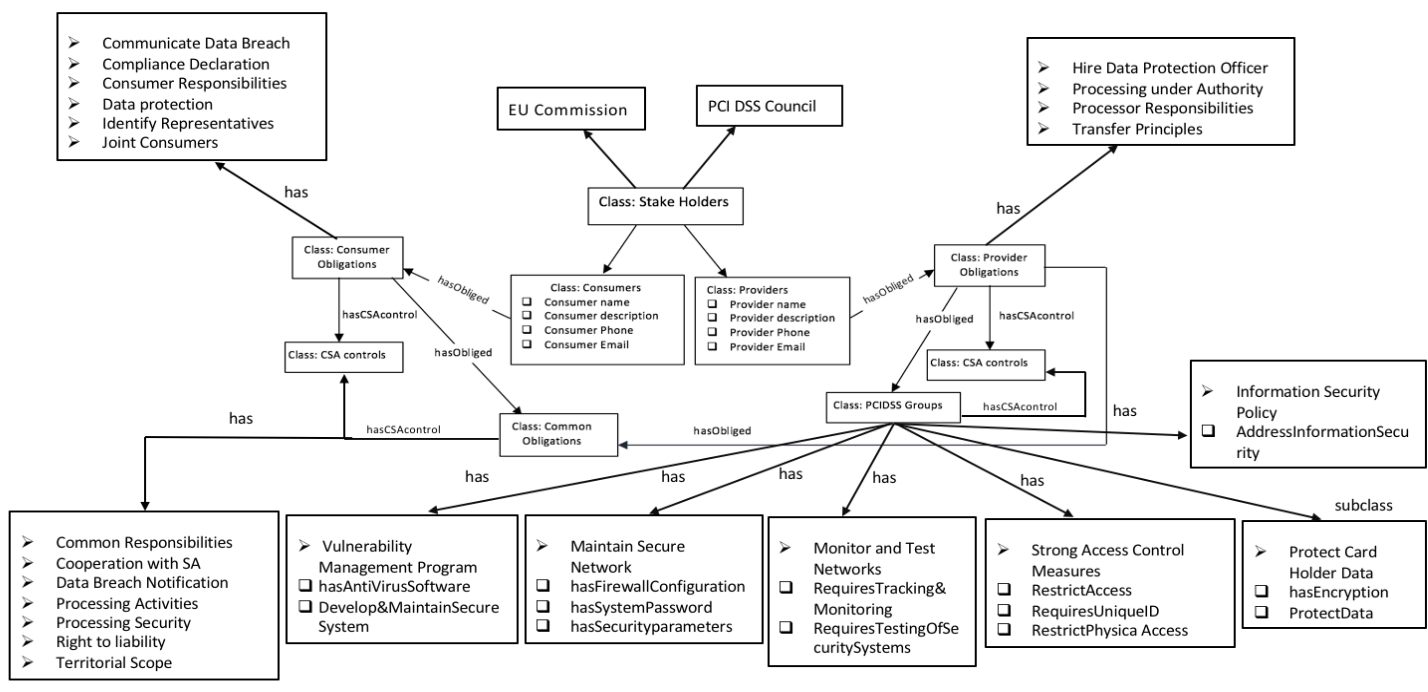
\includegraphics[width=\linewidth]{img/Elluri_ontology.png}
    \caption{Ontology of GDPR, PCI DSS, and CSA by Elluri et al. \cite{elluri_integrated_2018}}
    \label{fig:Elluri-ontology}
\end{figure}

The ontology development methodology included the following three steps: (i) Preprocessing, (ii) Ontology Development, and (iii) Validation. The preprocessing stage consisted of extracting relevant chapters and concepts from the text of the GDPR, PCI DSS, and CSA - and representing them using a preliminary ontology. These were then mapped with corresponding terms from the CSA ontology. This stage also involved identifying data protection rules in the form of permissions, obligations, dispensations, and prohibitions by using a keyword-based approach. Matching of concepts and rules was performed based using a tool that utilised text extraction and regular expressions to match contents with developed ontologies.

The validation of ontology utilised privacy policies of cloud service providers by comparing their text with the developed ontology using the developed tool. The extracted terms from policies were populated as instances of concepts in the developed ontology to provide an RDF representation of the policy. Apart from this description, the papers do not provide further details of the semantic representations or examples of the extracted information, nor an use-case demonstration of its capabilities. The ontology is referenced to be public and accessible\footnote{\url{https://ebiquity.umbc.edu/resource/html/id/377/Ontology-for-EU-s-General-Data-Protection-Regulation-GDPR}} \cite{elluri_knowledge_2018}, though it does not provide documentation or examples of its usage. Analysing the ontology shows instances of relevant chapters and articles within the GDPR applicable to PCI DSS and CSA, and declared as generic resources without reference to the actual text or IRI of the GDPR.

Related work within the same project by Joshi and Banerjee  \cite{joshi_automating_2019} concerns use of ontology to represent personal data categorisations and data privacy policies for automated enforcing of access control mechanisms regarding sharing of data with third parties through a blockchain. The data privacy policy, depicted in \autoref{fig:Ellur-PII-policy}, shows the concepts and relationships utilised to define information regarding processing. The privacy policy contains information about data collection purpose, data collected, protection measures, use limitations, consent requirements, and access control.
\begin{figure}[htbp]
    \centering
    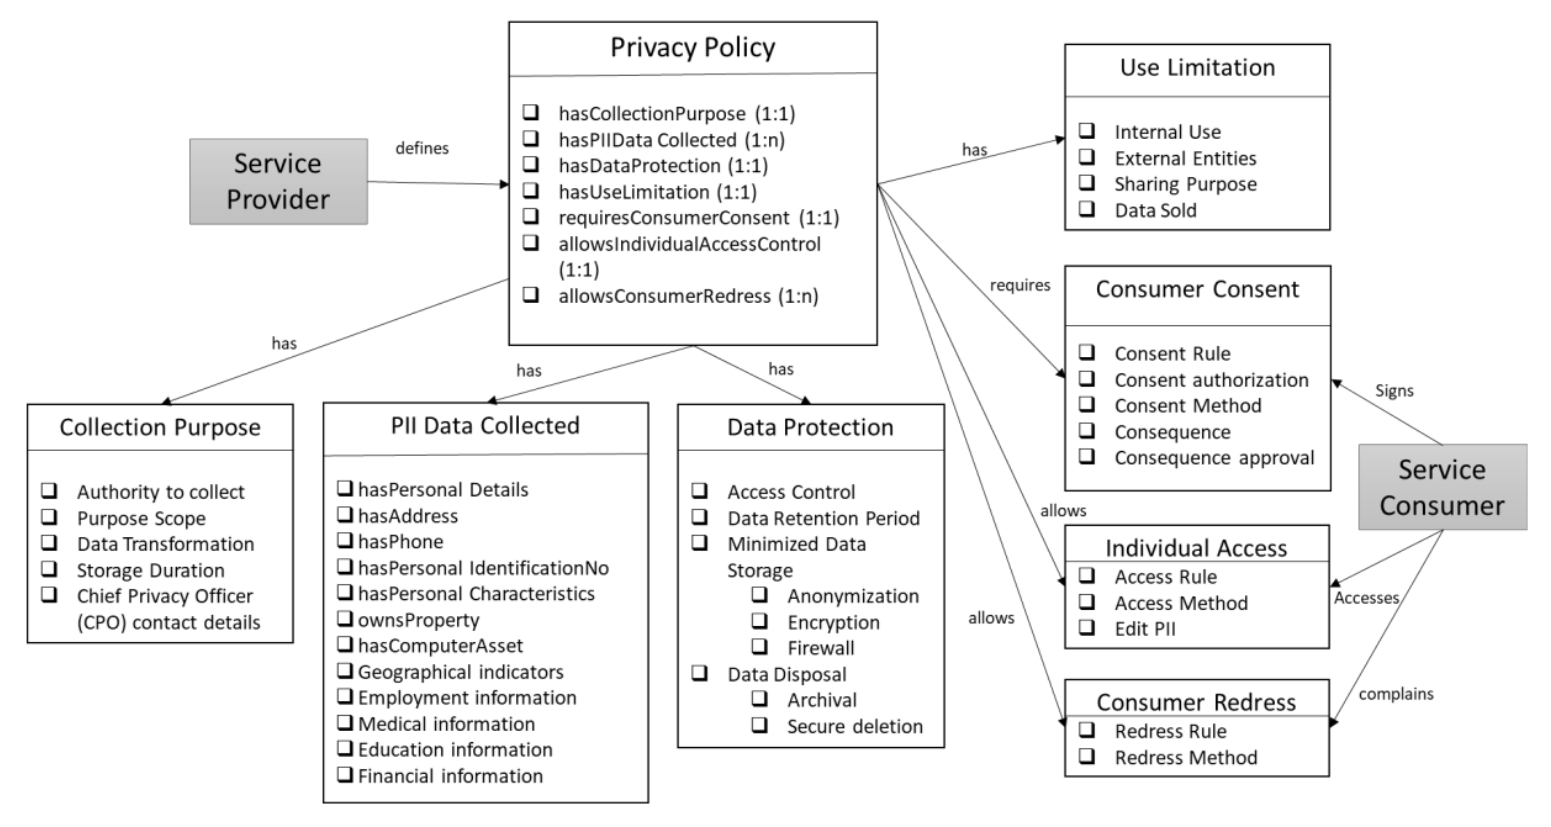
\includegraphics[width=\linewidth]{img/Elluri_PII_policy.png}
    \caption{Data Privacy Policy by Joshi and Banerjee \cite{joshi_automating_2019}}
    \label{fig:Ellur-PII-policy}
\end{figure}

The modelling of concepts includes some notably different relationships, such as the association of storage duration within collection purpose, usage limitation relating to data recipients, attributes associated with consent, and the inclusion of redress as a related concept. The developed ontology is utilised to extract and represent instances from privacy policies, enhance it using a reasoner, and to store the resulting access control representations in the blockchain. The work is based on the approach of utilising an existing privacy policy as a smart contract in the sharing of data between provider and consumer.
It is important to note that the work relates to the use of PII as opposed to personal data as defined by the GDPR. Furthermore, the policy does not encode information about rights as required by the GDPR.

\subsubsection{Ujcich et al.}\label{sec:sota:gdpr-semweb:ujcich}
Ujcich et al \cite{belhajjame_provenance_2018} presented a data provenance model of the GDPR which utilises PROV-O \cite{lebo_prov-o_2013} to represent activities and data in a semantic-web representation.
The data model provided in the publication is depicted in \autoref{fig:Ujcich-ontology} provides an overview of the concepts and uses PROV-O \cite{lebo_prov-o_2013} symbols to denote concepts.
The approach uses the activity `\textit{Justify}' to represent the rationale for processing personal data and has annotations depicting its starting and ending times, as well as a `\textit{Justification}' - which represents the legal basis of processing. The ontology focuses on the workflows involving exercising of rights under the GDPR, and provides examples of data rectification and withdrawal of consent utilising provenance.
\begin{figure}[htbp]
    \centering
    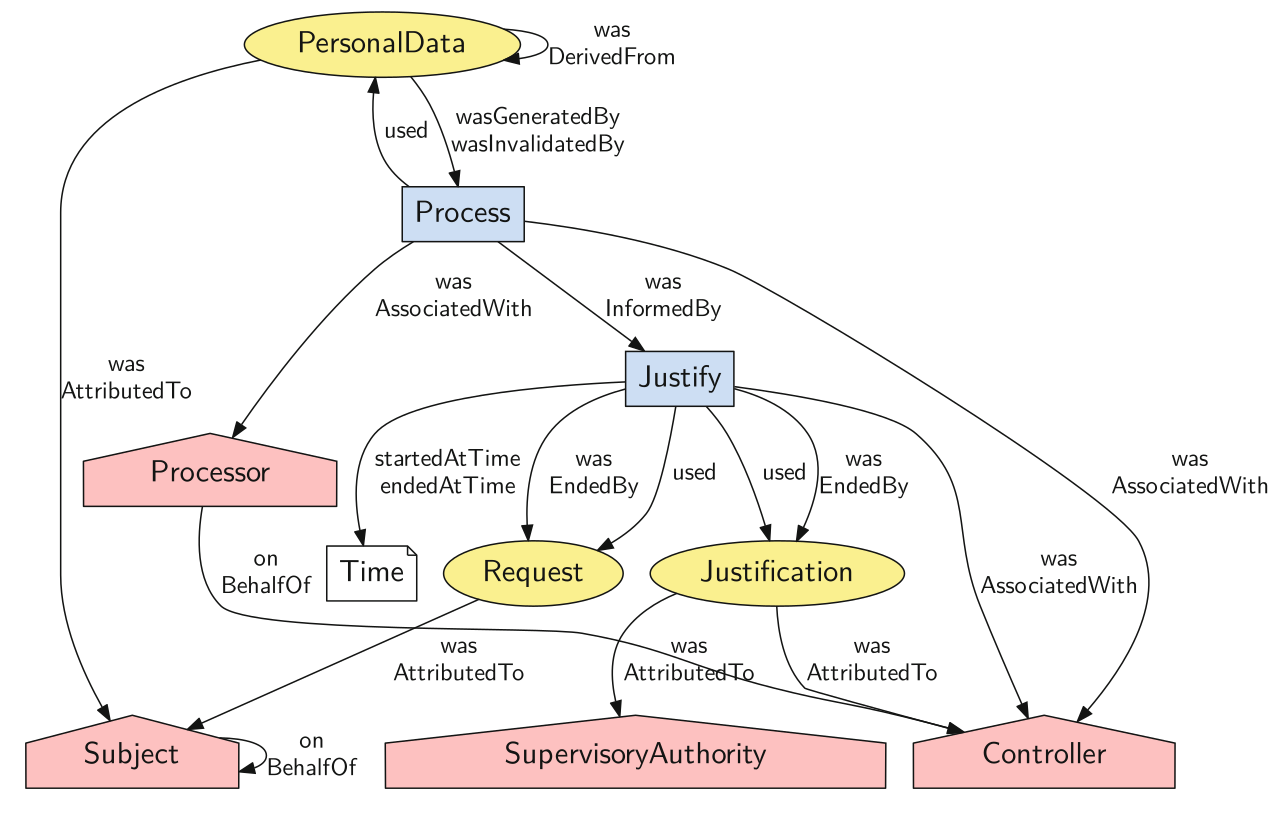
\includegraphics[width=\linewidth]{img/Ujcich_ontology.png}
    \caption{GDPR Data Provenance Model by Ujcich et al. \cite{belhajjame_provenance_2018}}
    \label{fig:Ujcich-ontology}
\end{figure}

The approach presented in the publication uses the notion of design patterns to describe the use of ontology in specific cases regarding the exercising of rights. The design pattern for provenance associated with consent does not associate the data directly with the consent owing to the reason of the data being potentially updated independent of consent. The design pattern is further extended to represent sharing data with a processor for marketing. The publication also provides a discussion on the verification of compliance based on provenance through questions which can be queried over the data represented using the presented ontology.

Specifying purposes as defined by GDPR is not clarified in this approach, as the concept of \textit{Justify} is temporal in its use and limited to the processing of personal data it is associated with. The approach also does not provide any information on modelling of more complex processing operations where more than one legal basis could be present, or a processing operation needs to be expressed in several steps. The approach also does not model information about consent or rights, and does not provide ex-ante representations of activities.

\subsubsection{Personal Information Controller Service (PICS)}
PICS is a project with the objective of enabling users to discover and control use of their personal data by utilising the platform as an authentication and management layer between service providers and personal information. The project architecture \cite{winckler_personal_2019} consists of three components: (i) personal data controller - provides an user interface allowing users to connect and mediate data to third-party services, (ii) ToS analyser - interprets terms of service and policies of providers using an ontology, and (iii) data mining traces of use - which enables discovery of web services utilising personal data shared with the service provider. The platform delegates the data storage to an external storage and does not store personal data itself. Authentication is performed at every interaction, and requires the user to provide physical authentication using a wearable device.

The ontology used by the ToS analyser \cite{benfenatki_towards_2018} consists of concepts associated with actions on data (such as deletion, disclosure, fusion, sharing), governance (laws, ownership, rights, terms of service), security strategies, and data protection. The ontology itself is not public or accessible and the publication does not provide complete details about its concepts or use beyond that of utilisation in the ToS analyser.

\subsubsection{ADvoCATE}
ADvoCATE \cite{rantos_advocate_2019} is a consent management platform for data processing in IoT that uses blockchain to record given consent, detects conflicts in data sharing policies, and provides recommendations for managing unwarranted exposure of personal data. In ADvoCATE, the consent notary component is responsible for obtaining and verifying consent signed by both the controller and the data subject, which is used to prepare a smart contract for processing based on the given consent. The consent management component then utilises the smart contract to update the user policy used to enforce access control over the stored personal data. Blockchain is utilised to store versioned hashes of consent linked to the smart contracts enforcing them. This enables traceability of consent and maintaining a record of consent and its relevant actions through the utilisation of smart contracts.
ADvoCATE has two components - Intelligent Policies Analysis Mechanism (IPAM) and Intelligent Recommendation Mechanism (IReMe) - to identify contradictory rules and policies regarding consent and adapt privacy strategies in real-time. 

A reference implementation describe in the publication uses the ontology of GDPR concepts by Bartolini et. al \cite{bartolini_using_2015} to model data protection requirements, and uses Ethereum as a blockchain platform, and Solidity for programming smart contracts. Examples of consent requests presented contain information about personal data category with collection medium and period, retention period, purpose, recipients (EU/Non-EU), whether it involves - automated processing, profiling, manual processing, and the IDs for controller, device, and device type.

\subsubsection{Ontology by Geko \& Tjoa}
Geko \& Tjoa \cite{geko_ontology_2018} proposed an ontology for capturing the interdependence between GDPR and information security requirements for assisting with compliance requirements involving security.
The ontology, depicted in \autoref{fig:Geko-ontology}, consists of hierarchical concepts representing the obligations of the GDPR and information security.
It has concepts regarding entities (Controller, Processor, Data Subject), rights, principles, personal data, obligations, and security. These are related using properties associated with fulfilling roles and obligations, ensuring data security, and provision of rights.
\begin{figure}[htbp]
    \centering
    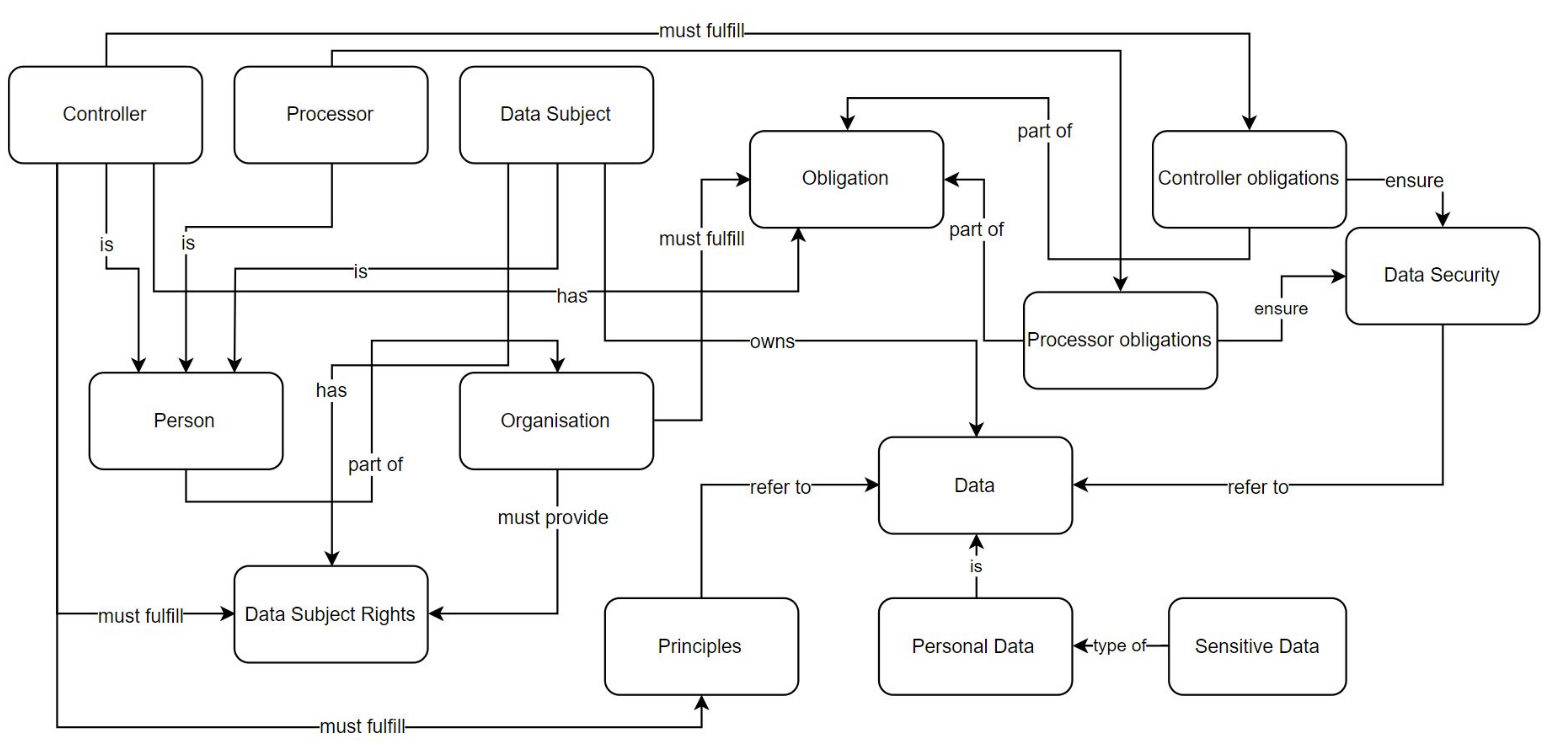
\includegraphics[width=0.8\linewidth]{img/Geko_ontology.png}
    \caption{Ontology for GDPR and Information Security by Geko \& Tjoa \cite{geko_ontology_2018}}
    \label{fig:Geko-ontology}
\end{figure}

The publication describes an example use-case of the ontology where additional concepts are added to represent security concepts of access control, audits, data classification, information risk assessment, security awareness, and security policy. Further concepts are also mentioned for representing technical measures of encryption, logging, network security, physical security, privacy by design and default, and pseudo-anonymisation.
The publication explicitly mentions that the ontology has not been evaluated. The publication also does not provide access to the ontology or its documentation.

\section{Other approaches addressing GDPR compliance}\label{sec:sota:gdpr-other}

\subsubsection{Layered Privacy Language (LPL)}
LPL \cite{gerl_lpl_2018} presents a formal model for specification of legal requirements regarding consent, data provenance, data retention and other privacy related concepts associated with the GDPR.
The objective of LPL is to be used in technical systems as a machine-readable privacy policy to provide privacy by design. 
LPL defines the following requirements for a privacy language: (i) differentiation between data-source and data-recipient to enable fine-grained access-control; (ii) modelling of purpose-based privacy policies with modelling of data, retention and anonymisation enabling privacy models; (iii) layering of privacy policies to ensure provenance; and (iv) human-readability.

The LPL structure, depicted in \autoref{fig:LPL-model}, consists of \textit{LayeredPrivacyPolicy} (LPP) as the root element representing a privacy policy or a legal contract. The element contains attributes for recording version information and an URI to the privacy policy containing its human-readable description. Each LPP can refer to an \textit{UnderlyingPrivacyPolicy} to enable tracking of privacy policies across multiple entities.
LPP is associated with a data source and its use in (multiple) purposes. The purpose is further associated with data recipients, data, privacy models, and data retention.
\begin{figure}[htbp]
    \centering
    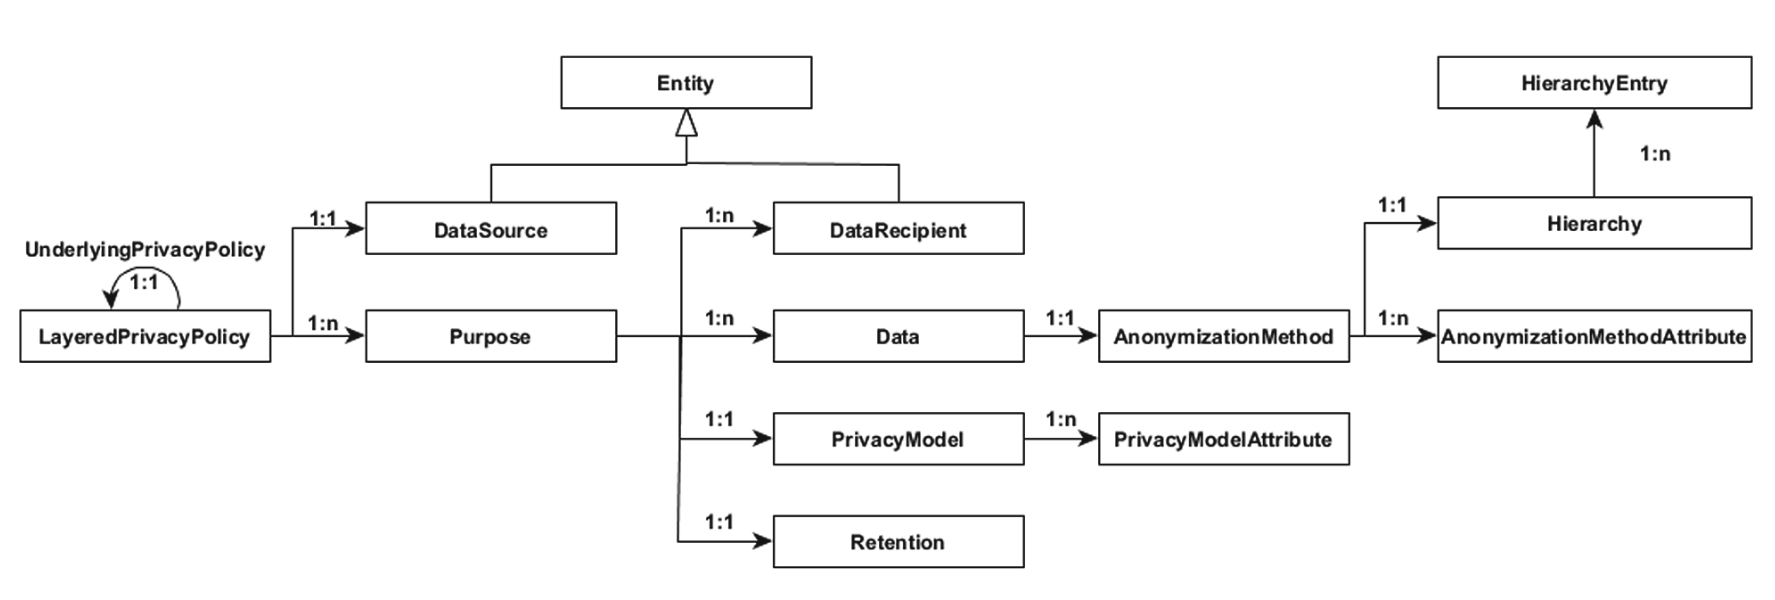
\includegraphics[width=\linewidth]{img/LPL_model.png}
    \caption{GuideMe approach by Ayala-Rivera and Pasquale \cite{gerl_lpl_2018}}
    \label{fig:LPL-model}
\end{figure}

LPL contains the concept of \textit{Entity-Hierarchy} where permissions provided to a parent entity can be controlled at a granular level with its child entities. An example of this is different departments within an organisation. Similarly, \textit{Purpose-Hierarchy} represents trees of purposes where a child purpose inherits the rights from a parent purpose. In this hierarchy, \textit{Regulated Purpose} specify a purpose required or obligated by the law.
Authorisation of entities and purposes is carried out by searching for rules matching the entity and purpose or their parents in the hierarchy. 

A critical analysis of the LPL for Article 12-14 of the GDPR was carried in the context of the work \cite{gerl_critical_2018}. This analysis presented requirements identified in the article of the GDPR and the corresponding LPL concepts along with whether they fulfil the stated requirements.
The analysis is used to present proposed changes to the LPL to incorporate additional concepts that fulfil the requirements.

\subsubsection{Lodge et al.}
Lodge et al. \cite{garcia-alfaro_developing_2018} present the Databox application development environment (SDK) for developing IoT apps utilising requirements to meet GDPR compliance. The SDK is provided with the objective to simplify compliance by utilising provided tools and design patterns.
The approach is based on identifying applicable requirements from the text of the GDPR and classifying them as based on risk or transparency.

The SDK enables modelling of applications as information flows consisting of four node types: data-stores - devices or services that generate data, processors - nodes that operate on data, profiler - nodes that infer new information about data subject, and outputs - nodes that perform action on data. Using the SDK, application developers can inspect ongoing risk breakdowns based on developed application, and track personal data as its moves through the application. The SDK also enables creation of GDPR-compliant contracts that embed the required information to provide informed consent, and provide automatic tooling for runtime data flow inspection.

Risks are detected based on whether the data is exported out of the platform, or triggers physical actuation, utilises insecure hardware, or uses unverified libraries. Tracking of personal data is provided by enforcing all outputs from a node to provide a personal data schema, which consists of top-level attributes associated with description of personal data, its source, and sensitivity.

GDPR compliant contracts are created by utilising the information flows to construct an agreement that is presented to the user. The agreement is visualised as a multi-layered notice that represents information taken from a manifest file containing all possible configurations in terms of data collection and usage. Developers can mark an information as compulsory or optional to indicate its basis in consent.

\subsubsection{Consent and Data Management Model by Peras}
Peras \cite{peras_guidelines_2018} presented 10 guidelines for implementing a consent management framework based on the requirements of the GDPR. These guidelines are based on adopting the requirements of consent and provision of rights in a data management system. The publication presents an analysis of existing consent and data management models\footnote{One of the works cited in this analysis is an approach developed in collaboration by the author \cite{fatema_compliance_2017} which acted as a precursor to the ontology developed to represent consent and presented in \autoref{sec:voc:GConsent}.} where the elements and attributes of the model are used for comparison. Based on this, a consent and data management model, depicted in \autoref{fig:Peras-model}, is proposed consisting of a contact interface for interactions between controllers and data subjects, a consent management module, a context management module, a data management module, and origin management.
\begin{figure}[htbp]
    \centering
    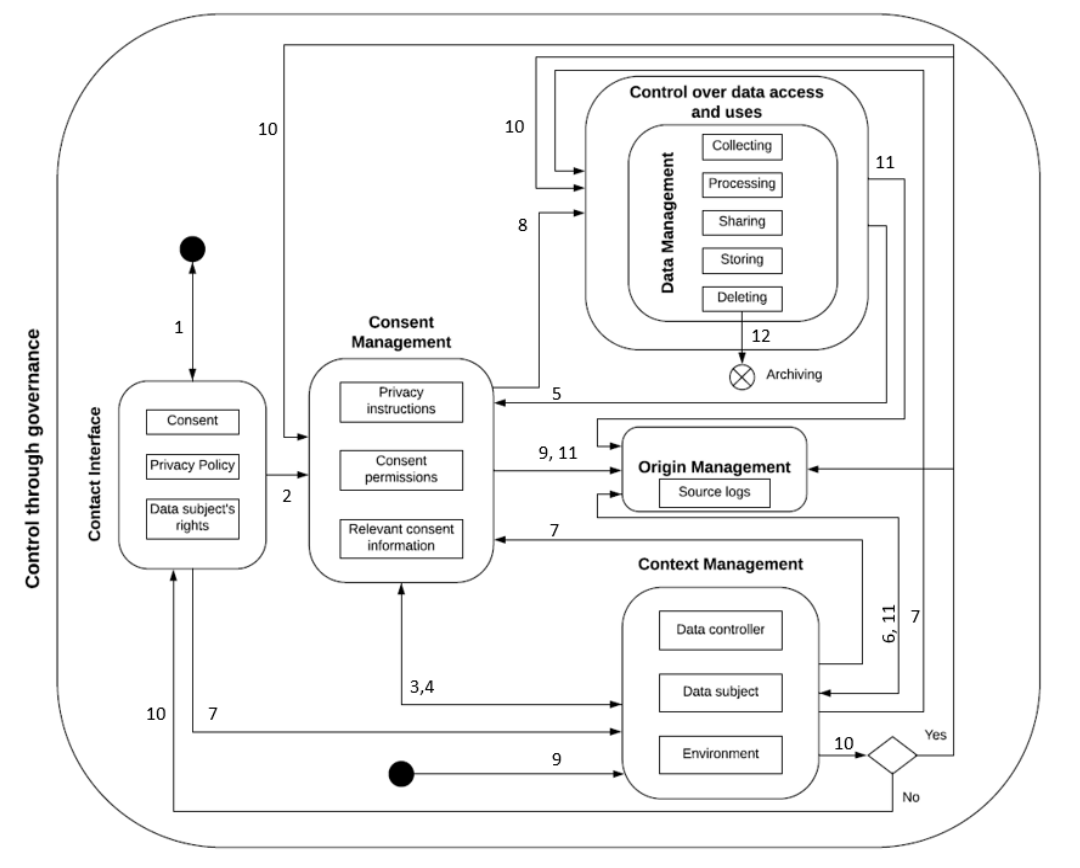
\includegraphics[width=0.8\linewidth]{img/Peras_model.png}
    \caption{Consent and Data Management Model by Peras \cite{peras_guidelines_2018}}
    \label{fig:Peras-model}
\end{figure}

\subsubsection{Tom et al.}
Tom et al. \cite{tom_conceptual_2018} presented a conceptual model of the GDPR representing the entities, actions, artefacts, rights, and their interactions. The publication provides a table of GDPR articles and their related entities and associations within the model, which it uses for evaluating completeness.
The model, depicted in \autoref{fig:Tom-model}, contains concepts regarding consent, purpose, data processing, technical measures, and actors such as controller, processor, data subject, and supervisory authority.
\begin{figure}[htbp]
    \centering
    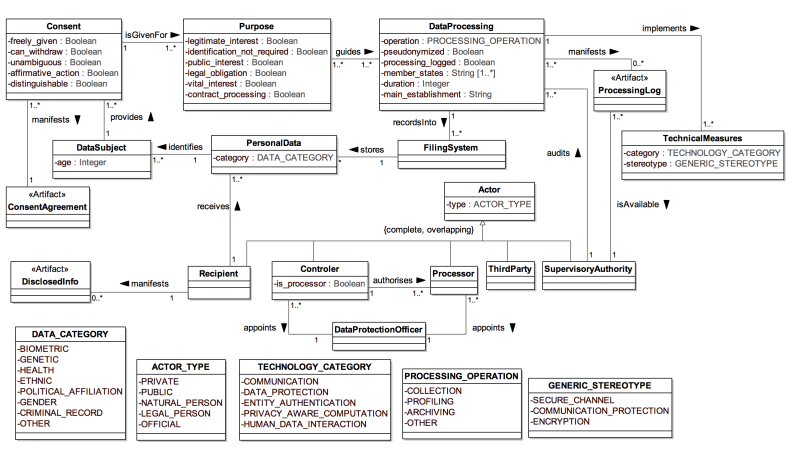
\includegraphics[width=\linewidth]{img/Tom_model.png}
    \caption{Conceptual Model of GDPR by Tom et al. \cite{tom_conceptual_2018}}
    \label{fig:Tom-model}
\end{figure}

The attributes of each concept are modelled based on database schemas, and represent conditions or additional information associated with the concept. For consent, boolean attributes define whether it was freely given, can be withdrawn, is unambiguous, was in affirmative action, and is distinguishable. Similarly, purpose has boolean attributes regarding whether it is in legitimate interest, does not require identification, is in public interest, for legal obligation, of vital interest to the data subject, and whether it indicates contract of processing. Certain attributes can refer to a table of concepts or instances, such as the \textit{PersonalData} attribute of category referring to \textit{DATA\_CATEGORY}. The publication provides examples of personal data categories, actor types (private, public, natural person, legal person, official), technology categories, processing operations, and generic stereotypes (secure channel, communication protection, encryption).

The model was utilised to develop an approach for analysing GDPR compliance over business process models using BPMN \cite{pullonen_privacy-enhanced_2019}.
The approach, termed PE-BPMN (Privacy Enhanced BPMN) and depicted in \autoref{fig:Tom-PEBPMN}, utilises BPMN to capture Privacy Enhancing Techniques (PETs) for capturing information flows. The approach is utilised in a mobile app scenario to analyse information disclosure.

The information disclosure analysis is performed based on identifying whether an object (personal data) is disclosed, which in this context is defined by it being received or intercepted by another party regardless of intent or policy. Objects can be visible, accessible, or hidden - based on whether the actor obtains and owns them, whether the data is protected or requires additional permissions, and whether it is protected by some PETs. The associated publication \cite{pullonen_privacy-enhanced_2019} presents details of an implemented prototype and its application in use-cases involving secure storage of data using encryption and PETs. 

The approach is similar to the use of semantic web ontologies to represent concepts and use of a semantic reasoner to evaluate compliance, such as in SPECIAL (\autoref{sec:sota:SPECIAL}). The use of BPMN differentiates the approach from other semantic representations of information, and the analysis provides a limited evaluation of compliance based on disclosure of personal data. While the approach contains concepts for representing information associated with how personal data is processed, it does not provide evidence of its use in evaluating other requirements of compliance - such as analysis of consent, or investigation of activities associated with sensitive personal data.
\begin{figure}[htbp]
    \centering
    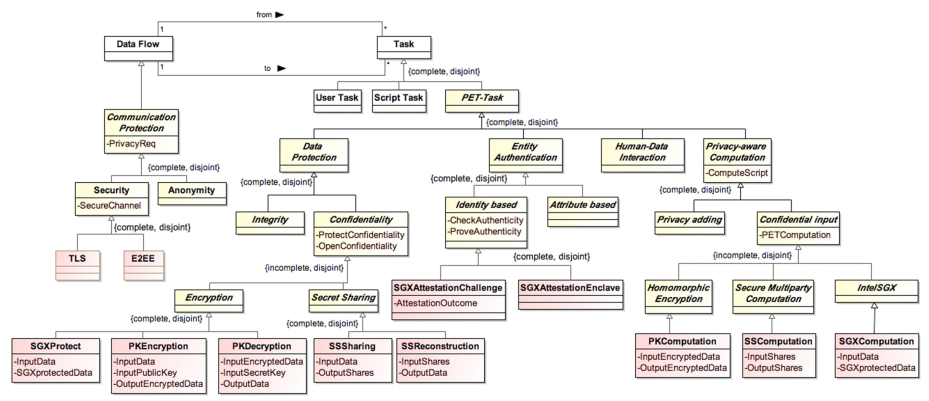
\includegraphics[width=\linewidth]{img/Tom_PEBPMN.png}
    \caption{PE-BPMN approach by Pullonen et al. \cite{pullonen_privacy-enhanced_2019}}
    \label{fig:Tom-PEBPMN}
\end{figure}

\subsubsection{Coletti et al.}
Coletti et al. \cite{kurosu_design_2019} proposed visual design patterns to provide transparency regarding personal data processing in mobile applications. These design patterns consist of recommendations for user interface and experience regarding providing information about processing and rights as per the requirements of the GDPR. Their approach identifies relevant information to be provided for transparency - which includes: (i) contact information for Controllers, Processors and Data Protection Officers, (ii) information about purpose of use, legal basis, and rights, (iii) Information about location as a specific form of data and processing, (iv) information about actions and algorithms utilised in processing, (iv) data sources, and (v) period of use and storage of data.

The visual design patterns organise this information into different layouts and screens to provide a simpler view to the data subject. A `springboard' consisting of an overview of the different sections is provided through which the information about each topic can be obtained. The approach recommends a three-layered approach consisting of - (1) purpose, legal basis, and rights; (2) subgroups of information such as specific laws related to legal basis, actionable tasks regarding rights; and (3) textual information with a search field.

\subsubsection{Corrales et al.}
Corrales et al. \cite{corrales_smart_2019} propose embedding legal requirements in smart contracts as a programmatic algorithm based on encoding the answers to a questionnaire into a compliance framework for data processing in the cloud. The questionnaire contains a set of 15 questions related to legal and technical issues including privacy, data protection and data security. The answers to the questionnaire are boolean in that they consist of affirmative (YES) or negative (NO). The algorithm for compliance then checks whether the questions have been answered in a way that meets the requirements of the GDPR. The pseudo-code presented in the publication consists of a series of steps checking whether the answers which can also be visualised in the form of a flow-chart containing decision making steps.

The approach is based on assessment of a questionnaire response rather than analyses of process representations. While the questions used are useful in the investigation of compliance, the approach does not provide any guideline or assistance regarding gathering information required to answer them, or even evaluating the information apart from the boolean response.

\subsubsection{LUCE}
LUCE \cite{havelange_luce_2019} (A Blockchain Solution for monitoring data License accoUntability and CompliancE) is a platform for facilitating compliance with licensing terms by enabling data accountability through recording of data use and purpose using blockchain. The platform specifically aims to provide compliance assistance towards the GDPR and its rights. LUCE has the following objectives: (i) to automatically manage and enforce licensing terms attached to a dataset, ii) record and makes available information pertaining to how and for which purpose the dataset is reused, and iii) enable compliance with the GDPR rights regarding data access, rectification, and erasure. The architecture, depicted in \autoref{fig:sota:LUCE-architecture}, consists of four layers for management of metadata, entities, data, and blockchain. 
\begin{figure}[htbp]
    \centering
    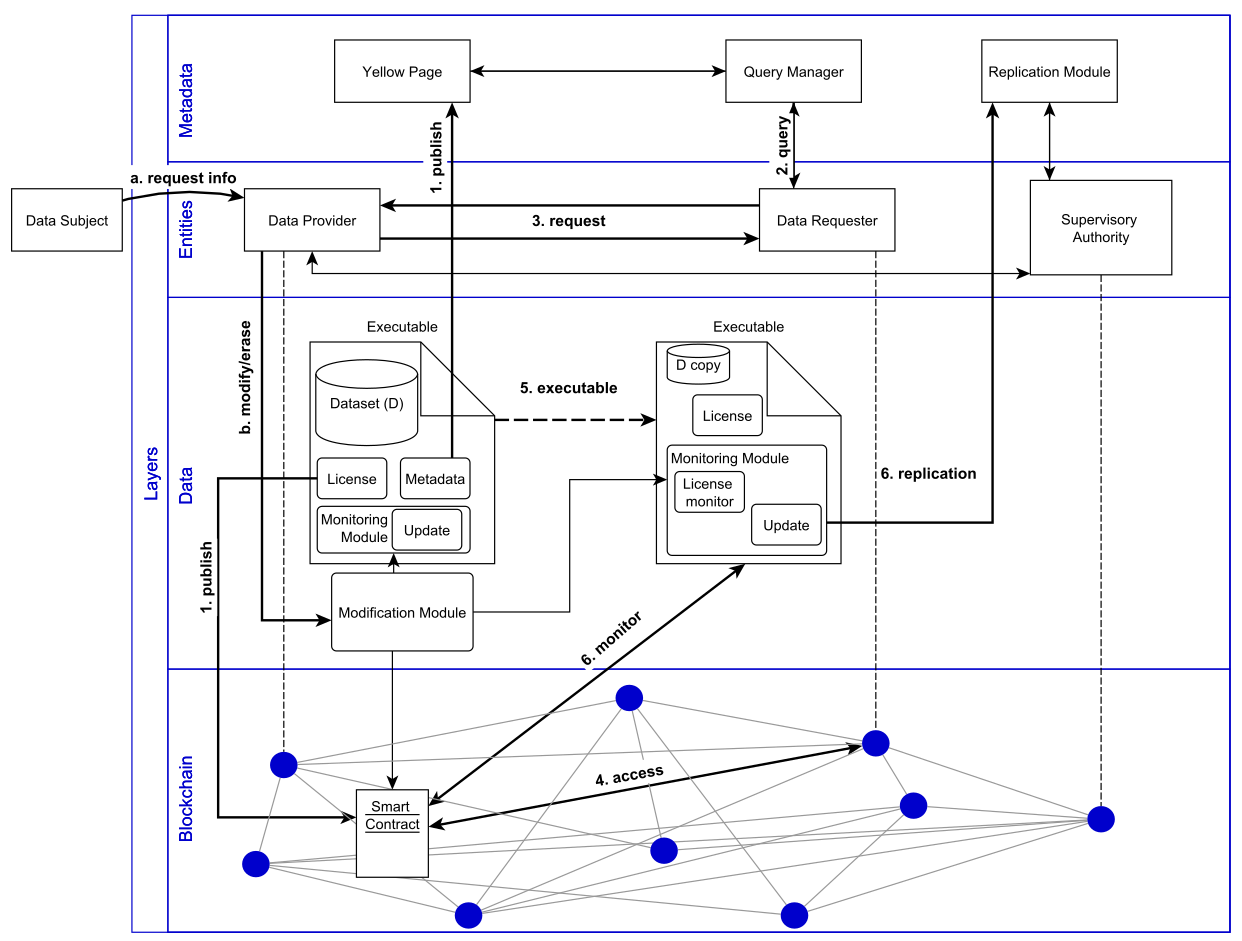
\includegraphics[width=0.8\linewidth]{img/LUCE_architecture.png}
    \caption{Architecture of LUCE \cite{havelange_luce_2019}}
    \label{fig:sota:LUCE-architecture}
\end{figure}

Data providers publish their dataset metadata into a \textit{Yellow Page} shared directory where requestors can search for matching datasets. Each dataset is accompanied with licensing information for access and reuse to the data. A transaction for reusing data is implemented in the form of a smart contract which contains the associated license as an obligation of terms. Requestors accepting the licensing agreements are provided with an access token which is tracked within the smart contract for compliance. The \textit{License-Monitoring} sub-module continuously checks the actions performed by the data requester comply with the licensing terms and records these actions in a file which constitutes a log of events. Access tokens are valid for a specific time period, after which renewal is granted based on prior compliance with the licensing terms, which are checked using the event logs. A data provider can also check accesses to the data and the status of requestor's compliance. GDPR rights are enforced and supplemented by using the smart contracts to perform actions, such as retrieving information to provide regarding right to access, and obtaining IDs for deletion regarding right to erasure and rectification. The prototype implementation described uses Ethereum\footnote{\url{https://ethereum.org/}} as the blockchain platform and Solidity\footnote{\url{https://solidity.readthedocs.io/}} as the smart contracts language.

\subsubsection{Decision Provenance by Singh et al.}
Singh et al. propose the concept of `Decision Provenance' - which uses methods based on provision to identify decision pipelines and actions taken in an system at design and run-time. 
Decision provenance is aimed to facilitate oversight, audit, compliance, risk mitigation, and user empowerment, and relates to the accountability of algorithmic systems.
The paper provides a discussion of GDPR, identifying the legal impetus to identify and record provenance information regarding processing of personal data and management of rights. 
The utilisation of data flows in a system to map actions, steps, and boundaries is utilised as motivation for its use in a compliance management system based on adapting legal requirements over the design and use of such data flows. With this, `decision provenance' is defined as ``use and means for provenance mechanisms to assist accountability considerations in algorithmic systems''.

The information required to be recorded and utilised for decision provenance concerns the history or provenance of data, and a broader view of system behaviour and interactions including those with entities. The publication also describes the usefulness of such information in ex-post analysis.
Regarding compliance, decision provenance is described with uses for tracking of conditions associated with processing, consent, purposes, rights, and sharing.
The collected information is also described for uses in performing audits and investigations by authorities as well as the organisation itself.

The publication makes specific mention of PROV \cite{lebo_prov-o_2013} for representing provenance information, supplemented by ontologies for describing additional information about data processing.
An example cited in this context concerns the use of PROV-O to represent provenance for GDPR compliance (Ujcich et al. \cite{belhajjame_provenance_2018} - see \autoref{sec:sota:gdpr-semweb:ujcich}).

\subsubsection{Sion et al.}
Sion et al. \cite{sion_architectural_2019} presented an approach for data protection by design in software architectures towards incorporating the requirements of GDPR. The approach is developed towards automation of data protection impact assessment (DPIA) using (i) meta-model constraints, (ii) model analysis, and  (iii) interaction with stakeholders. It uses architectural notations, such as UML and Data Flow Diagrams (DFD) to express the model of a system.  The publication provides a discussion of necessary information for the creation of a meta-model for GDPR, which includes the following:
\begin{itemize}
    \item Use of GDPR terminology as opposed to abstract architectural notations; 
    \item Core abstractions such as \textit{ProcessingPurpose};
    \item Documentation regarding abstractions - such as collection, further processing, the purpose itself, its legal basis (termed \textit{LawfulGround}), involved actors and their roles, and datasets and data-types involved for a purpose.
\end{itemize}

The presented meta-model, depicted in \autoref{fig:sota:Sion-model}, utilises UML to denote the concepts and their relationships. Apart from expressing concepts such as purpose, processing, personal data type, and data subject type, the meta-model expresses controllers, processors, recipients and third parties as legal roles expressed through an actor. Additionally, it has a distinct concept for further processing to represent processing other than that of the primary purpose. Exceptions to the obligations provided by GDPR are captured as prohibition and exemption types.
\begin{figure}[htbp]
    \centering
    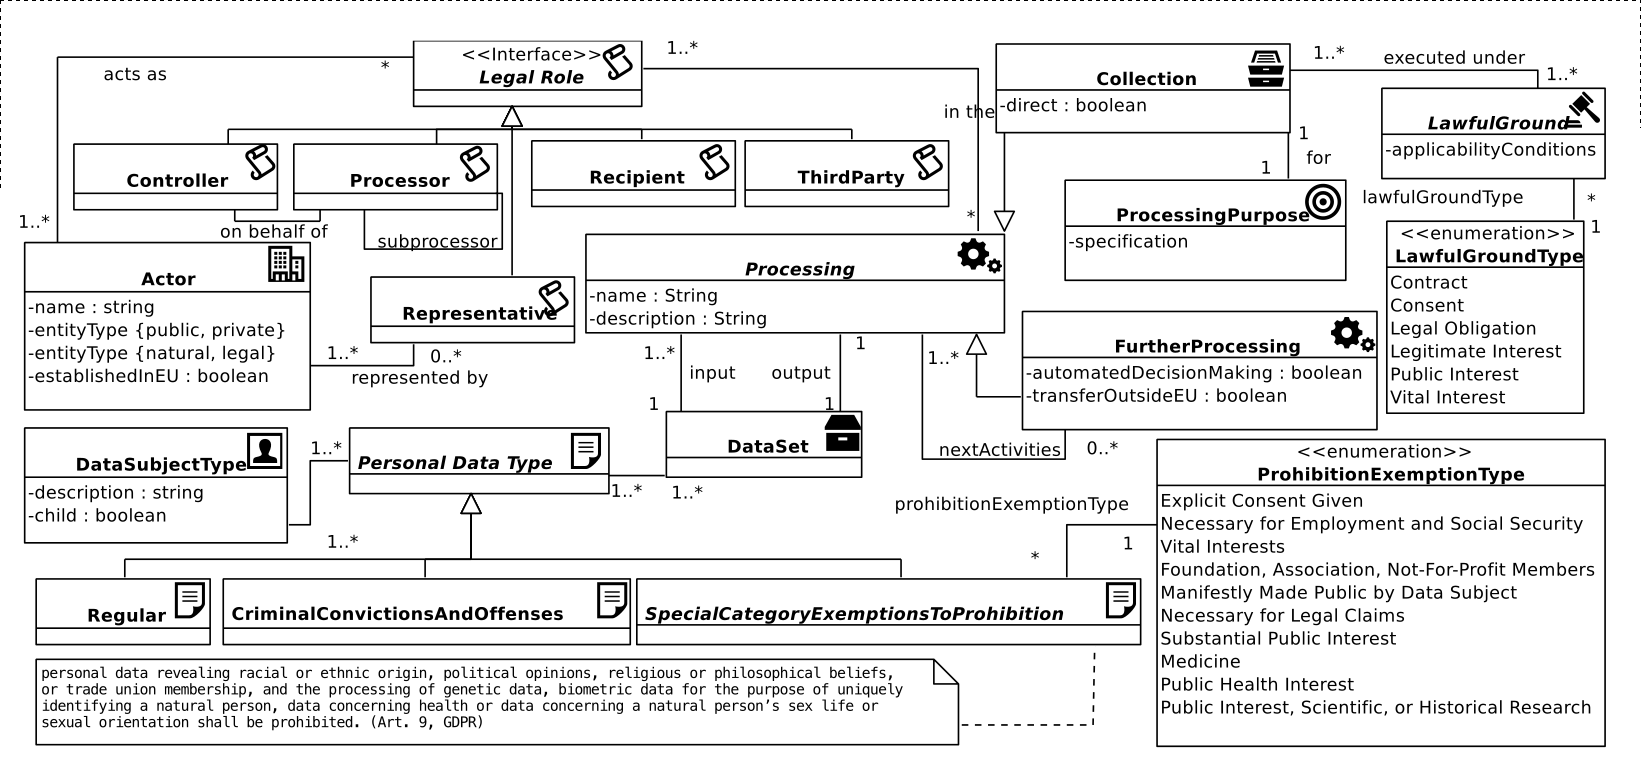
\includegraphics[width=\linewidth]{img/Sion_model.png}
    \caption{Meta-model of architectural view for GDPR by Sion et al. \cite{sion_architectural_2019}}
    \label{fig:sota:Sion-model}
\end{figure}

The meta-model is used to express the model or architecture of a system, which is then evaluated or validated utilising a number of constraints. One of these, described in the publication, is ``soundness criteria'' - which is relevant to the completeness and correctness of a model. Examples of these are - ``every chain of Processing needs to start with a Collection'', and ``Every input DataSet to a Processing needs to be the output DataSet of a Processing that is located earlier in the chain of Processings''. These can be collectively expressed as constraints for every data used in processing to have a source whether by collection or as output of processing activity. The publication also provides examples of incorporating legal requirements over the meta-model, with examples for purpose limitation, minimisation, and automated decision making involving special categories of personal data. 

The approach is validated through an use-case in the health domain involving a patient monitoring system (PMS), using DFD to denote architectural notations in Eclipse Modelling Framework, with graphical visualisations created using Sirius viewpoint specification. The soundness checks were performed using the Acceleo Query Language supported by Sirius, with work in progress for implementing compliance assessment rules using VIATRA’s graph-based pattern language

\subsubsection{privacyTracker}
or privacyTracker \cite{gjermundrod_privacytracker_2016} is a framework that provides data traceability through privacy by design principles for GDPR compliance. The framework utilises policies to mediate access to information stored in the form of \textit{Customer Records}, and consists of 3 modules regarding data collection, data distribution, and data traceability. The \textit{Customer Record} is a XML document utilising XSD to store personal data, and contains two sections - a mandatory metadata section and an optional section. The metadata section contains fields for record identification, data tractability, and cryptography controls. The optional section consists of fields indicating public data, private data which can be disclosed based on consent, and data provided by enterprise itself.

The record identification field contains a URI based on string concatenation of company name, user email address and auto-generated random identifier. This URI is unique throughout the framework, but changes when the data is distributed to another entity. In addition, the identification field also stores timestamps associated with record genesis, (local) record creation, and expiration. The data tractability fields record links to the entity that generated the record (backward-to-root reference), entities the record was obtained from (backward reference), and entities the record is disclosed to (forward reference). The cryptography controls store a signed copy of the received record and a signature in the form of hash code of the complete record.
The distribution module enables sharing of data via an API through which granular requests can be made. Records of distributions are signed cryptographically and verified for tractability.
Enforcing rights is simplified by traversing the stored distribution records starting from the original record as root and moving towards the leaves.
A prototype of the implementation consisted of 6 companies and used MySQL and PHP as the technological framework. The records were stored using XML, which was then ingested into the database and queried using SQL.

The analysis of GDPR presented in connection with privacyTracker provide a list of requirements required to be satisfied by compliance frameworks, which are: Articles 5(1a), 5(1d), 6(1a), 6(1c), 7(1), 7(3), 12(1), 12(2), 14(1a), 14(1ac), 14a(2g), 15, 16(1), 17(1), 17(2a), 17a(1), 18(2), 19(2)). These provide the obligation to record and demonstrate evidence regarding handling and sharing of consumer data. 

\subsubsection{Metrics for Transparency by Spagnuelo et al.}
Spagnuelo et al. \cite{livraga_metrics_2016} define eight quality metrics for transparency regarding data processing associated with the GDPR.
In this context, transparency is defined based on quality factors of Informativeness, Understandability, and Accessibility associated with providing information, and Validity and Accessibility associated with providing mechanisms.
Each metric is associated with one or more questions that retrieve information regarding quality factors associated with its quantitative scoring.
The metrics provide a quantifiable representation of transparency in a system, and are used in a use-case to evaluate Microsoft Health-Vault - a commercial product.
The metrics are as follows - accuracy, currentness, conciseness, detailing, readability, availability, portability, and effectiveness.

\subsubsection{Metamodel for PLA by Diamantopoulou et al.}
Diamantopoulou et al. present a metamodel for representing Privacy Level Agreements (PLA) with the aim of establishing contracts between controllers and individuals.
The metamodel, depicted in \autoref{fig:Diamantopoulou-metamodel}, represents privacy preferences using the concept of questionnaires, where each question refers to a specific data and the answer represents the individual's preferences regarding data sharing. The metamodel also associates preferences with threats, risks, and security measures through the data and controller. Requests for sharing data are associated with data and preferences, and can be accepted or denied based on the values of linked preferences.
The metamodel is specified to be designed for use-case in eGovernance scenarios where public administrators can provide data and value based on citizens preferences represented through the metamodel.
\begin{figure}[htbp]
    \centering
    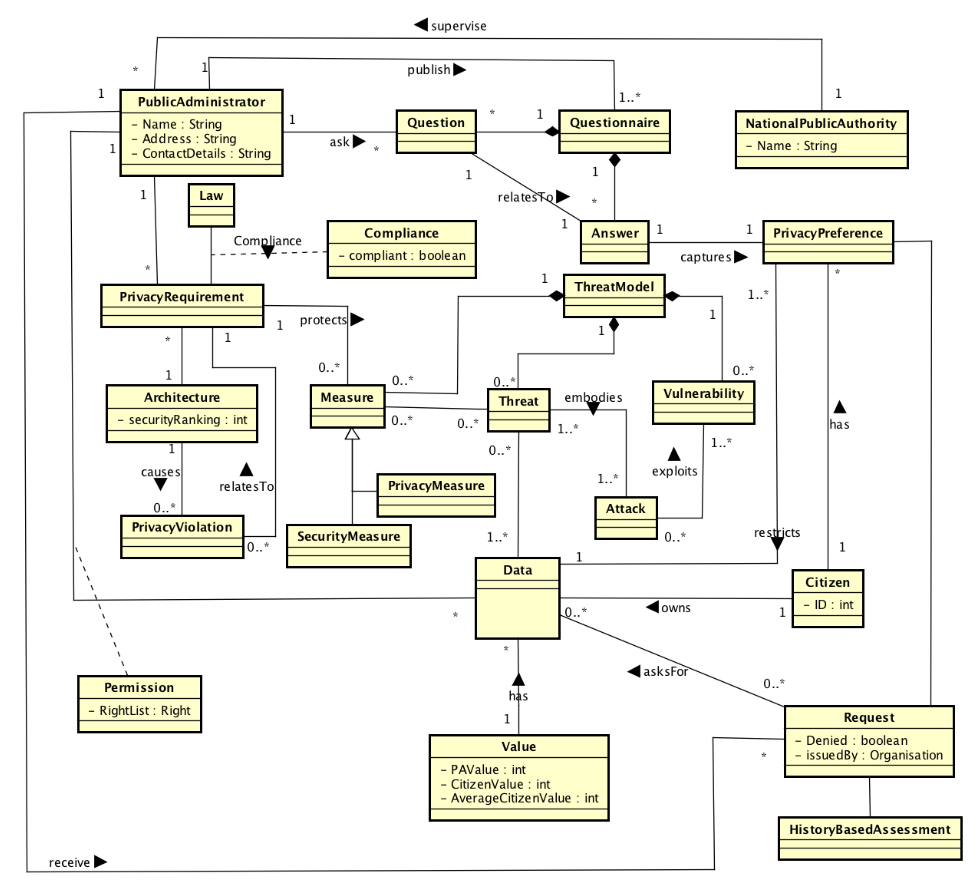
\includegraphics[width=0.8\linewidth]{img/Diamantopoulou_metamodel.png}
    \caption{Metamodel for Privacy Level Agreements by Diamantopoulou et al. \cite{diamantopoulou_metamodel_2017}}
    \label{fig:Diamantopoulou-metamodel}
\end{figure}

\subsubsection{Robol et al.}
Robol et al. \cite{robol_toward_2017} proposed a modelling and reasoning framework based on socio-technical systems \cite{dalpiaz_security_2016} - an approach for incorporating interaction between people and technology. The proposed framework extends STS-ml - a goal-based modelling language provided in STS - with relevant concepts regarding privacy by design and GDPR compliance. The extended modelling language consists of three views - social, information, and authorisation - based on concepts and context of interactions between them. Social views incorporate actors and their goals and documents, as well as delegations and transmissions. Information views consist of associating actors with information and the tangible documents. Authorisation views consist of interactions with actors based on authorisations which are validated by legal basis over some information towards a particular goal. The modelling concepts are explained in the publication using a health-domain use-case.

Reasoning is based on using the concepts in policies that are then validated for compliance. The policies are based on formal representations of rules based on conditions and constraints for compliance, and the notion of \textit{well-formedness} of models. One notable aspect of this work is the use of concepts from socio-technical approaches to represent GDPR concepts. In particular, goal is used to simulate purpose, actors are used to conceptualise individuals and controllers, and authorisation is used to simulate valid legal basis. The approach enables use of STS modelling and reasoning to develop rules for expressing GDPR compliance requirements and validations.

\subsubsection{Basin et al.}
Basin et al. \cite{basin_purpose_2018} proposed an approach that aligns purpose as defined by the GDPR with a business process, and uses formal models of inter-process communication to audit GDPR compliance. The approach also uses models of data flows to derive privacy policies. 
The definition of business process used in the approach consists of having a set of activities that take inputs and produce outputs, have a beginning and an end, and are ordered. The inter-process communication is based on the understanding of data-flow graphs where different processes interact and share the same set of data for different purposes.

The auditing mechanism in the approach is based on validating whether an implementation conforms to process collections i.e. implemented activities conform to modelled processes, process collection conforms to privacy policy i.e. modelled processes conform to those specified within a privacy policy, process collection conforms to GDPR, and privacy policy conforms to GDPR.
The process collection is defined as a tuple $PC = (P,D,DU,DC)$ consisting of processes ($P$), data classes ($D$), data usage ($DU\subset D x P$), and data collection ($DC\subset D x P$). Consent is based on evaluating whether the process collection permitted by consent falls within that defined by the privacy policy. Similarly, data minimisation is evaluated by assessing whether all data collected is utilised in some process.

% \subsection{GDPR Privacy Label}
% GDPR Privacy Label \cite{fox_communicating_2018} - GDPR privacy label - creating a privacy label to inform data subjects about the data processing characteristics such as identity of controller, purposes, recipients, transfers, consent - withdrawal

% non sem-web
\subsubsection{RestAssured}
RestAssured\footnote{\url{https://restassuredh2020.eu/}} is an European H2020 project that aims to enable secure data processing in the cloud with sticky policies for decentralised data lifecycle management.
The project aims to achieve this by using run-time models for data protection assurance and automated risk management. Run-time detection, prediction, and prevention of data protection violations is achieved by using a catalogue of risk patterns representing data protection vulnerabilities of cloud systems \cite{palm_modelling_2018,braubach_using_2018}. The pattern meta-model and its validation is described in detail in the deliverable D5.1 \cite{noauthor_d5.1_2018}. Information about the project is available through peer-reviewed publications and publicly available deliverables\footnote{\url{https://restassuredh2020.eu/publications/}}.
\begin{figure}[htbp]
    \centering
    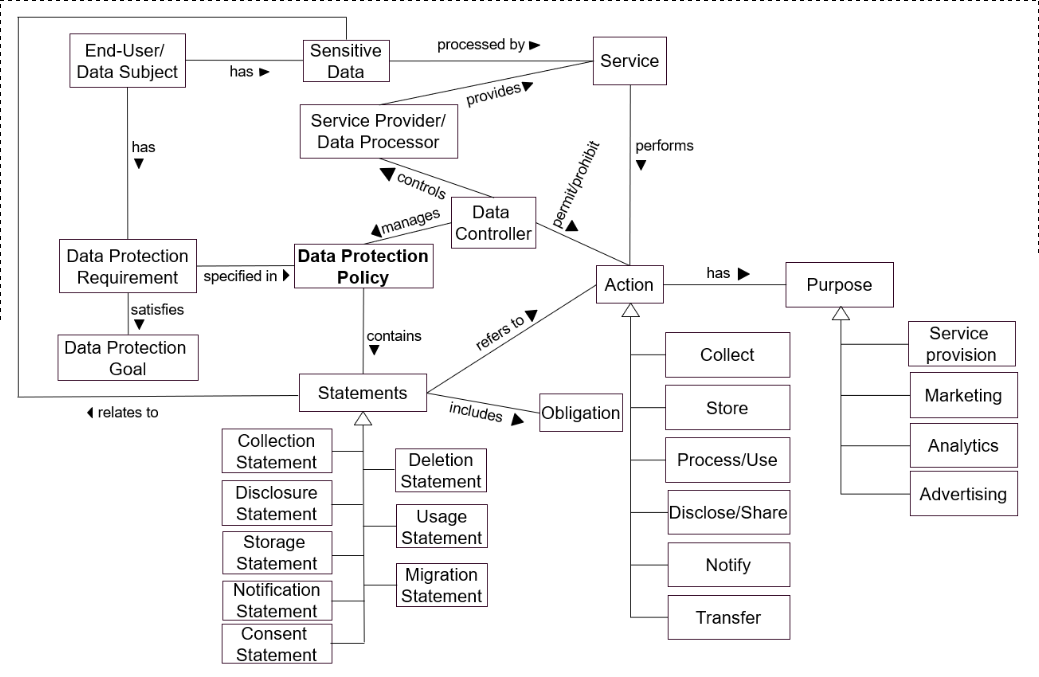
\includegraphics[width=\linewidth]{img/RestAssured_model.png}
    \caption{Model of policy specification framework in RestAssured \cite{RestAssured_D6.1}}
    \label{fig:RestAssured-model}
\end{figure}

% non sem-web
The project addresses GDPR specifically through a conceptual model incorporating concepts necessary for compliance, as depicted in \autoref{fig:RestAssured-model} \cite{RestAssured_D6.1}. The model is utilised in a data protection policy specification consisting of a data protection contract, sticky policies, and specification of obligations. The model is utilised to provide a customised privacy policy that allows users choice of preferences for selected services \cite{gritzalis_privacy_2019}. The data protection contract is composed of 4 main parts - description of the Service that needs to access the data, specification of the data that is needed to be accessed by the service and whether this access is mandatory, list of usages where usage is composed of a textual description that describes the purpose of this usage and the associated processing action as well as a list of needed data types, and specification of data that will be published by the service.
The obligations are defined based on their enforcement in relation to access control (before, at same time, after), and are specified with three pieces of information: (i) obligation type (before, after, with), (ii) event trigger, and (iii) action to be performed. The serialisation of obligations is done using XACML 3.0.
The deliverable D7.1 \cite{noauthor_d7.1_2018} refers to the use of RDF to represent the concepts and relationships as a graph, which consists of three layers representing: (i) a core model of the schema that captures the fundamental concepts, e.g. assets, roles, threats, and their relationships; (ii) a domain model of datasets that encode domain- specific knowledge, e.g. detailed threats and their possible control strategies; and (iii) system models that represent an actual system upon which the risk assessment is being performed.

% non sem-web
\subsubsection{OPERANDO}
OPERANDO\footnote{\url{www.operando.eu/}} (Online Privacy Enforcement, Rights Assurance \& Optimisation) is an European H2020 project that aims to provide a platform for users to specify preferences via a dashboard, which is then compared with online service providers privacy policies and converted into access control rules.
The deliverable D3.1 \cite{noauthor_d3.1_2016} describes the legal requirements of the GDPR in the context of OPERANDO's objectives, while deliverable D6.4 \cite{noauthor_d6.4_2017} describes the architecture and working of privacy tools.
Information about the project is available through peer-reviewed publications and public deliverables\footnote{\url{http://www.operando.eu/servizi/moduli/moduli_fase01b.aspx}}.

The platform operates in an online environment and uses APIs between services which pass information using JSON. An User Privacy Policy (UPP) \cite{noauthor_d6.7_2017} is stored in the platform database and represents the user's preferences (and consent). The UPP records preferences using fields for information identifiers, personal data category, ranked preference (0 to 10, higher indicating greater concern), role (of person acting on data), action (performed on data), purpose, and recipient. The UPP also contains information on access policies created based on comparing the user's preferences against an online service provider's privacy policy. 

The online service provider's privacy policy (OSP) \cite{noauthor_d6.7_2017} consists of fields defining workflows and contained steps with information about requester subject (role of service provider), requested data, and action to be performed. The OSP also contains information about access policies for which the service provider has privileges to perform the requested operations in specified roles. Information about how the UPP and OSP are utilised in an API to enact an access request is provided through the deliverable D6.4 \cite{noauthor_d6.4_2017}.

% non sem-web
\subsubsection{My Health My Data (MHMD)}
My Health My Data\footnote{\url{http://www.myhealthmydata.eu/}} (MHMD) is an European H2020 project that aims to develop infrastructure based on blockchain and smart contracts, which provide personal data accounts in the cloud that can be managed using dynamic consent interfaces and provide peer-to-peer connections between stakeholders. The project uses blockchain to log data transactions in a secure, transparent, and accountable manner, while using de-identification and encryption to protect identity and sensitive information. The safety and security of the data is tested using re-identification and penetration simulations.
Information about the project is available through peer-reviewed publications and public deliverables\footnote{\url{http://www.myhealthmydata.eu/publicdeliverables/}}.

The project is applied over the use-case of health data and devices, described in deliverable D1.1 \cite{noauthor_d1.1_2017}, and uses an ontological resource to model the common data ontology - described more in its deliverable D4.2 \cite{teodoro_d4.2_2018}. The common data ontology consists of modular health data ontologies representing synthetic data shared by the project's commercial partners as an use-case.
Access to the data is provided through an API that includes parameters describing the requested data category as well as consent descriptions. The API returns matching datasets which can then be utilised for data processing activities. The consent description parameter of the API is a text field consisting of values such as ``synthetic data'' and ``fully anonymised'' which reflect the state of data and its requirements in terms of consent. 

Though the project aims to utilise the GDPR as a source of legal requirements and strives to design its framework to meet compliance requirements by both design and default, there is no publicly available information regarding the specifics of how GDPR compliance is achieved or represented.
It focuses on the privacy preserving and security aspects of data storage by using technological solutions such as access control and transparent logging to design specifications based on legal requirements.
The project does explores the impact of GDPR of storing data in a blockchain, especially regarding the right to be forgotten \cite{bayle_when_2018}.

\section{Approaches involving Privacy Policies}\label{sec:sota:privacy-policies}
These approaches involve utilisation of privacy policies for various purposes associated with data protection and user empowerment. While they do not target GDPR compliance, they are relevant to the work as they involve analysis of information associated with compliance - such as purposes, data categories, and rights - and also provide an overview of GDPR's impact and uptake in the real-world.

\subsubsection{Usable Privacy Project}
The UsablePrivacy project \cite{sadeh_usable_2013} utilised natural language programming over manually annotated corpus of privacy policies to create a system for automatic classification of policies. 
It utilised semantic web technologies \cite{oltramari_privonto_2018} to represent the annotations and information within a privacy policy, as well as to query information for retrieval.
The datasets generated as part of the project have been utilised in other similar approaches \cite{harkous_polisis_2018,linden_privacy_2018} concerning automatic analyses over privacy policies. 

\subsubsection{Polisis and other approaches based on Usable Privacy Project}
Galle et al. \cite{galle_case_2019} presented an argument for a similar corpus of GDPR-specific privacy policies based on the increased requirements required for GDPR compliance based on the presence of information and use of simpler text. While such a dataset has not been published to date, there have been approaches incorporating GDPR specific information in privacy policy analysis.
Polisis \cite{harkous_polisis_2018} is one such approach that analyses privacy policies using the taxonomy of privacy concepts by Wilson et al. \cite{wilson_creation_2016} (depicted in \autoref{fig:sota:Linden-taxonomy}).
Further GDPR specific work using the same approach collects and compares policies in pre-GDPR and post-GDPR versions to identify the impact of GDPR \cite{linden_privacy_2018}. The approach uses a list of the queries derived from ICO’s GDPR compliance checklists to obtain coverage of GDPR in terms of queries answerable in privacy policies.
\begin{figure}[htbp]
    \centering
    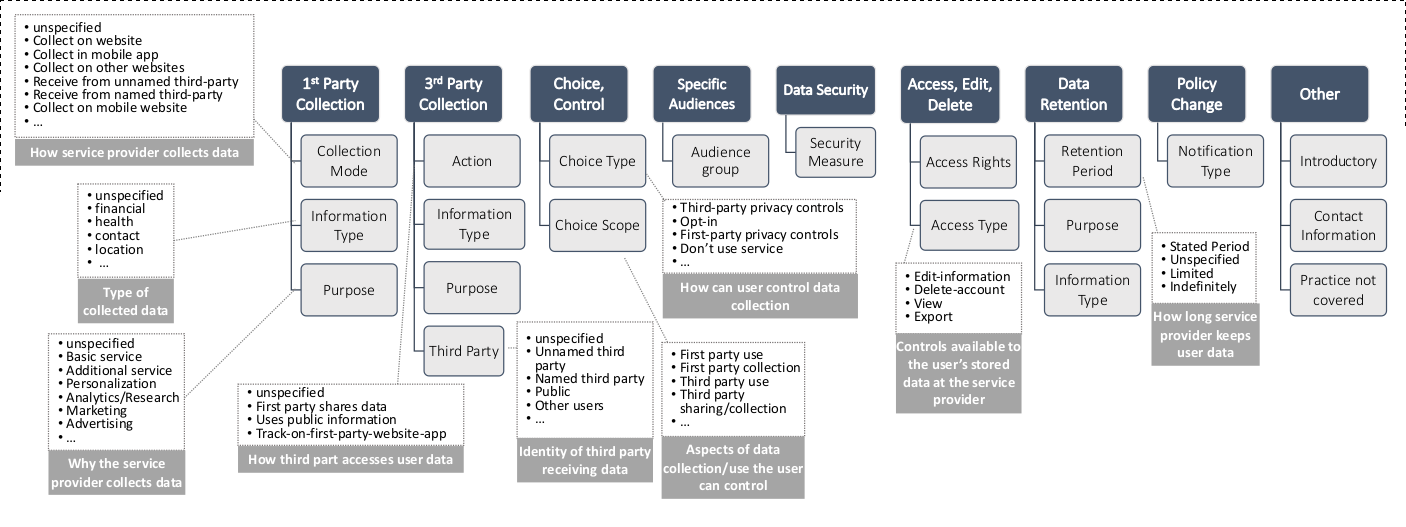
\includegraphics[width=\linewidth]{img/Linden_taxonomy.png}
    \caption{Privacy taxonomy by Wilson et al. \cite{wilson_creation_2016} used by Harkous et al. \cite{harkous_polisis_2018} and Linden et al.  \cite{linden_privacy_2018} to analyse privacy policies}
    \label{fig:sota:Linden-taxonomy}
\end{figure}

\subsubsection{PrivacyGuide}
PrivacyGuide \cite{tesfay_privacyguide_2018,westphal_spirit_2018} provides visualisation of privacy policies and information categories in the form of a dashboard. It uses a similar approach to UsablePrivacy and Polisis in classifying statements in policies and extracting information using machine learning. In terms of information, its models contain the following concepts: data collection, protection of children, third-party sharing, data security, data retention, data aggregation, control of data, privacy settings, account deletion, privacy breach notification, policy changes.
The approach is based on identifying a set of keywords for each concept and classifying statements based on their presence.

\section{Approaches related to Consent}\label{sec:sota:consent}
These approaches involve association with consent, and provide information about existing efforts towards its representation and analysis. They are relevant as they involve information associated with the provision of consent, its impact in real-life, and the complexities associated with its representations.

\subsubsection{Grando et al.}
Grando et al. \cite{grando_ontological_2012} present an ontology-based model of permissions and obligations resulting from informed consent within the medical domain. The approach, depicted in \autoref{fig:sota:Grando-ontology}, consists of using XACML for rules implementing a consent management system by utilising reasoning using SWRL.
\begin{figure}[htbp]
    \centering
    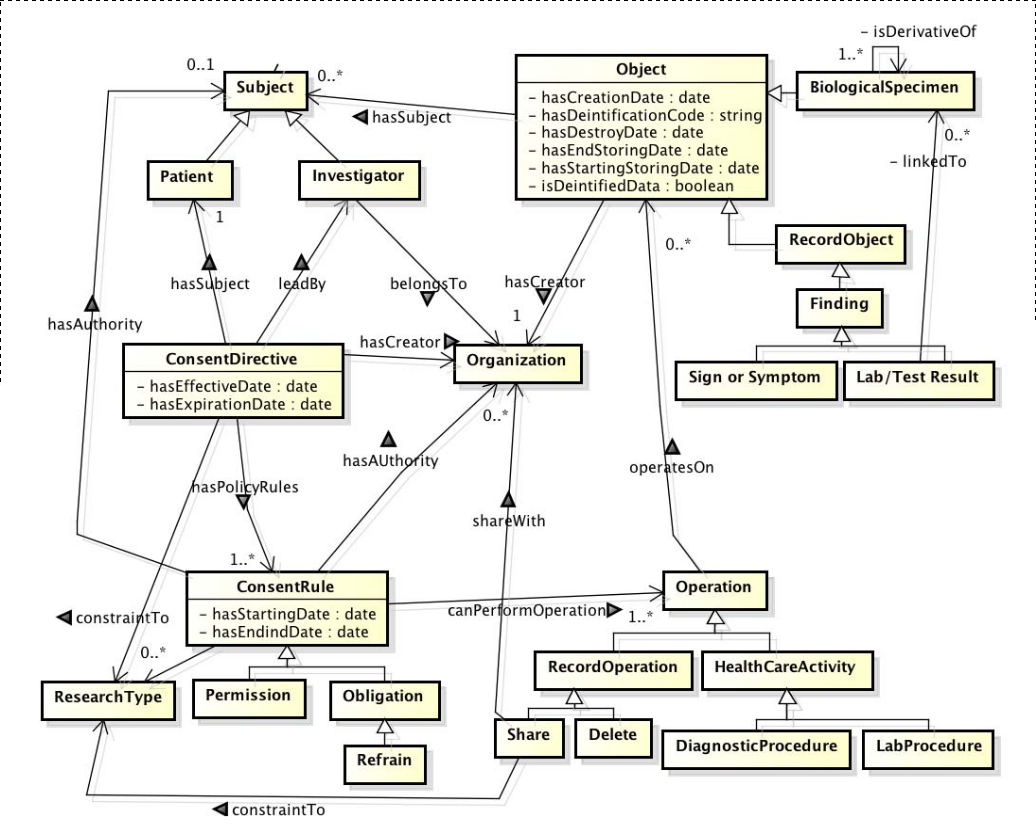
\includegraphics[width=0.75\linewidth]{img/Grando_ontology.png}
    \caption{Informed consent permissions ontology by Grando et al. \cite{grando_ontological_2012}}
    \label{fig:sota:Grando-ontology}
\end{figure}

\subsubsection{Consent Receipt Specification}
The Consent Receipt specification\footnote{\url{https://kantarainitiative.org/confluence/display/infosharing/Consent+Receipt+Specification}} \cite{lizar_consent_2017} is a standardisation effort by the Kantara Initiative - a non-profit industry professional trade association with the mission - ``improving trustworthy use of identity and personal data through innovation, standardisation and good practice in the domain of digital identity management and data privacy''. The consent receipt provides a list of fields necessary to capture the context of given consent and is meant to be a record of transaction regarding personal data. Its fields, depicted in \autoref{fig:sota:ConsentReceipt}, capture information about timestamp the consent was given at, the entities involved (controllers), PII involved, purposes, and recipients.
\begin{figure}[htbp]
    \centering
    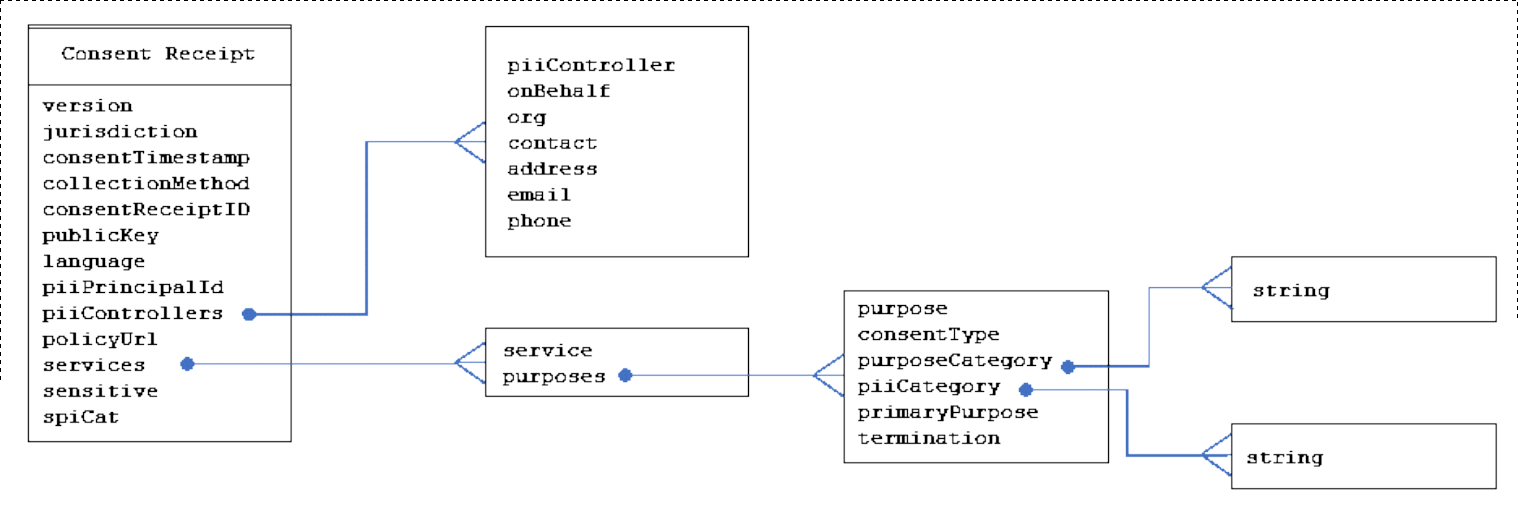
\includegraphics[width=\linewidth]{img/ConsentReceipt.png}
    \caption{Fields in Consent Receipt \cite{lizar_consent_2017}}
    \label{fig:sota:ConsentReceipt}
\end{figure}

\section{Upcoming research projects addressing GDPR}
This section lists upcoming research projects that address or incorporate GDPR compliance in their requirements and are currently developing solutions to meet their objectives and aims. These are presented to include them in the larger picture of approaches associated with GDPR compliance, but are not analysed as part of the SotA relevant to this thesis given their nascent research output.

\subsubsection{PDP4E}
PDP43\footnote{\url{https://www.pdp4e-project.eu/}} (Methods and Tools for GDPR Compliance through Privacy and Data Protection Engineering) is an European H2020 project that aims to provide tools and guidance for incorporating privacy and data protection into software development life-cycles (SDLC) to implement data protection by design. Currently, the project lists one deliverable on its website, D2.1 \cite{noauthor_d2.1_2019}, which provides information on the legal analysis of GDPR in terms of requirements and obligations for software, and identifies the various roles and responsibilities within the context of SDLC.

% non sem-web
\subsubsection{DEFeND}
DEFeND\footnote{\url{https://www.defendproject.eu/}} (Data Privacy Governance for Supporting GDPR) is an European H2020 project that aims to create a platform for providing services to organisations in the context of GDPR compliance. The platform is stated to provide services regarding data management and governance, data breach reporting, process management, along with GDPR planning and reporting. The peer reviewed publication \cite{piras_defend_2019} presents more details about the architecture of the project and its various components.

The Data Assessment Component (DAC) consists of the Organisation Data Collection (ODC) module which uses an questionnaire to collect information about organisational scope, data processing, processes, and activities - and is used to evaluate the organisation with relevant aspects of the GDPR. The questionnaire responses from ODC are given to the Assessment Translator (ATr) module which converts them to an XML-schema in order to create Data Assessment Model (DAM) - which is a goal-based requirement engineering model of actors, assets, establishments and data flows.

The DAM is used by the Data Privacy Analysis Component (DPAC) to perform analysis about DPIA, Data Minimisation, Privacy-by-Design/Default, and Threat mitigation. The outcome of the analysis is a Data Privacy Model (DPC), which is utilised to specify and evaluate both at design and run-time the operations of consent management, data access rights, security and privacy technologies. The project also aims to create a dashboard to provide organisations with control and monitoring of operations to achieve GDPR compliance, and to enable data subjects to interact with the platform based on consent.

% non sem-web, relevant
\subsubsection{PAPAYA}
PAPAYA\footnote{\url{https://www.papaya-project.eu/}} (PlAtform for PrivAcY preserving data Analytics) is an European H2020 project that aims to provide privacy preserving techniques and technologies for performing analytics tasks on encrypted data by untrusted third-party data processors. The project uses the obligations of the GDPR to structure its outcomes in terms of Privacy Enhancing Technologies (PETs) which are provided through an interoperable platform. The project focuses on the application of privacy by design principle to provide usability, transparency, and auditability to end users regarding the processing of their data. Information about the project is available through peer-reviewed publications\footnote{The deliverables listed at \url{https://www.papaya-project.eu/deliverables} are not publicly accessible at the time of writing this thesis.}.

% non sem-web, relevant
\subsubsection{SMOOTH}
SMOOTH\footnote{\url{https://smoothplatform.eu/}} is an European H2020 project that aims to assist micro enterprises become compliant with the GDPR by designing and implementing tools for awareness about GDPR obligations and analysing their level of compliance with the new data protection regulation.
The objectives of the project include creation of a platform for automatic assessment of privacy protection documents (including privacy policies), stored data, and the processing of personal data on the website or mobile apps to create a compliance report. Further details about the project are currently not available.

% non sem-web
\subsubsection{SODA}
SODA\footnote{\url{https://www.soda-project.eu/}} (Scalable Oblivious Data Analytics) is an European H2020 project that aims to provide tools for performing analytics over encrypted data at large scales while providing compliance with the GDPR. The project will utilise use-cases within the health domain to demonstrate the privacy-preserving aspects of its technologies. SODA incorporates requirements of the GDPR and provides guarantees regarding compliance through the use of its tools and technologies. The analysis of legal requirements arising from the GDPR and the role of SODA in addressing them is presented in deliverable D3.1 \cite{spindler_d3.1_2017}. Further information about the project is available through peer-reviewed publications and public deliverables\footnote{\url{https://www.soda-project.eu/deliverables/}}.

% non sem-web, relevant
\subsubsection{DECODE}
DECODE\footnote{\url{https://decodeproject.eu/}} is an European H2020 project that aims to provide tools for data ownership by using blockchain with attribute-based cryptography. The project will be piloted in Amsterdam and Barcelona, and will focus on enabling citizens to manage and control the data generated through IoT devices. The objective of the project is to provide the data as a shared resource for collective benefit and crowd-sourced information. Smart contracts are used to enable control of data and are stored in a distributed ledger (such as blockchain). Information about the project is available through its public deliverables\footnote{\url{https://decodeproject.eu/publications}}.

The specification of information required for legal compliance as well as processing is defined in terms of `entitlements', which include personal data category, description, purpose, condition (alternate purpose), expiry date (storage duration). These are collected across use-cases, normalised to find commonalities, and utilised in smart policies to record information about processing. The deliverable D3.5 \cite{roio_d3.5_2018} describes collected entitlements from use-cases in Barcelona pilot.
The analysis of legal requirements and their incorporation in the DECODE project is described in D1.8 \cite{noauthor_d1.8_2017}.
\subsubsection{MOSAICrOWN}
MOSAICrOWN\footnote{\url{https://mosaicrown.eu/}} (Multi-Owner data Sharing for Analytics and Integration respecting Confidentiality and OWNer control) is an European H2020 project that aims to enable data sharing and collaborative analytics in multi-owner scenarios. Its objectives are to provide a data governance framework able to capture and combine the protection requirements specified by multiple parties, and to provide protection techniques for enabling efficient and scalable data sharing and processing.
One of the outcomes of the research is an approach for performing combining selective encryption, blockchain, and smart contracts to enable data owners to leverage data markets to monetise their data in a con-trolled way. Our approach is complemented by an audit process counteracting misbehaviour in case of dishonest subjects.
% \subsubsection{MUSKETEER}

% non sem-web, relevant
\subsubsection{PoSEID-on}
POSEID-on\footnote{\url{https://www.poseidon-h2020.eu/}} (Protection and control of Secured Information by means of a privacy Enhanced Dashboard) is an European H2020 project that aims to safeguard the rights of data subjects
while simultaneously supporting organisations in data management and processing while ensuring GDPR compliance.
Its objective is to create a Privacy Enhancing Dashboard for personal data protection using an implementation of permissioned blockchain and smart contracts to provide accountability, transparency and compliance.
The project aims to develop technologies for automated detection of unexpected and potentially harmful behaviours in order to monitor privacy risks and notify threats to data subjects during transactions.
Information about the project is available through its public deliverables\footnote{\url{https://www.poseidon-h2020.eu/documents/}}.

Deliverable D2.1 \cite{noauthor_d2.1_2018} provides information on use-cases considered within the project with their user stories, personal data required in the use-case, and third parties involved. Deliverable D3.1 \cite{noauthor_d3.1_2019} presents the architecture of the PoSEID-on, with information about the smart contract utilised on the permissioned blockchain. The smart contract supports permissions regarding requesting, granting, revoking, notifying, checking, and accessing permissions regarding use of PII. Each permission event is logged to the blockchain and consists of the data processor, data subject, and personal data field involved. Deliverable D4.3 \cite{noauthor_d4.3_2019} describes use of natural language programming approaches to detect PII in stored data as a measure of risk detection and management.

\section{Analysis}\label{sec:sota:analysis}

\subsubsection{Overview of SotA}
The analysis of the state of the art was carried out using the methodology presented earlier in \autoref{sec:sota:methodology}.
The approaches were first analysed to identify their relevance for the categories of information identified in the methodology.
\autoref{table:sota:analysis:overview} presents this information by using a check mark (\cmark) to indicate the approach uses or provide information about that topic, with its absence indicating that the approach does not address that topic or no information about its use could be found.
The column headings represent the identified categories of information from the methodology, and represent the following - (T): type of work where PRJ indicates a research project and RES indicates research publication, (R): if it models GDPR clauses and concepts, (MG): if it provides an ontology, (EA): if it represents information for ex-ante Compliance, (EP): if it represents information for ex-post compliance, (P): if it models activities, (C): if it represents consent, (Cm): if it evaluates compliance, (Rq): if it specifies requirements for GDPR compliance, and (O): it provides resources in an open and accessible manner.
\begin{table}[htbp]
\footnotesize
\centering
\rowcolors{2}{}{gray!10}
\begin{tabularx}{\textwidth}{|l|X|X|X|X|X|X|X|X|X|X|}
\rowcolor{white}
\caption{Overview of approaches in SotA}\label{table:sota:analysis:overview} \\
\hline
\textbf{Work} & \textbf{T} & \textbf{R} & \textbf{M} & \textbf{EA} & \textbf{EP} & \textbf{P} & \textbf{C} &\textbf{Cm} & \textbf{Rq} & \textbf{O} \\ \hline
\multicolumn{11}{|>{\hsize=\dimexpr11\hsize+11\tabcolsep+12\arrayrulewidth\relax}X|}{Approaches using semantic web to address GDPR compliance} \\ \hline
SPECIAL & PRJ &  & \cmark & \cmark & \cmark & \cmark & \cmark & \cmark &  & \cmark \\ \hline
SERAMIS & PRJ & \cmark & \cmark &  &  &  &  & \cmark & \cmark &  \\ \hline
Vos et al & RES &  & \cmark &  &  &  &  & \cmark & \cmark & \cmark \\ \hline
CitySPIN & PRJ &  & \cmark & \cmark & \cmark & \cmark & \cmark & \cmark &  & \cmark \\ \hline
MIREL & PRJ & \cmark & \cmark & \cmark & \cmark & \cmark &  & \cmark & \cmark &  \\ \hline
DAPRECO & PRJ & \cmark & \cmark & \cmark & \cmark & \cmark &  & \cmark & \cmark &  \\ \hline
BPR4GDPR & PRJ &  &  & \cmark & \cmark & \cmark &  & \cmark & \cmark &  \\ \hline
Elluri et al. & RES &  & \cmark &  &  &  &  &  &  & \cmark \\ \hline
Ujcich et al. & RES &  & \cmark &  & \cmark & \cmark &  &  &  &  \\ \hline
PICS & RES &  &  &  & \cmark &  &  &  &  &  \\ \hline
AdvoCATE & RES &  & \cmark &  &  &  & \cmark & \cmark &  &  \\ \hline
Geko \& Tjoa & RES &  & \cmark &  &  &  &  &  &  &  \\ \hline
\multicolumn{11}{|>{\hsize=\dimexpr11\hsize+11\tabcolsep+12\arrayrulewidth\relax}X|}{Other approaches addressing GDPR compliance} \\ \hline
LPL & RES &  & \cmark &  &  &  &  &  &  &  \\ \hline
Lodge et al & RES &  & \cmark &  & \cmark & \cmark & \cmark & \cmark &  &  \\ \hline
Peras & RES &  & \cmark &  &  &  & \cmark &  &  &  \\ \hline
Tom et al & RES &  & \cmark & \cmark &  & \cmark &  & \cmark &  &  \\ \hline
Coletti et al & RES &  & \cmark & \cmark &  &  & \cmark &  & \cmark &  \\ \hline
Corrales et al & RES &  &  &  &  &  &  & \cmark & \cmark &  \\ \hline
LUCE & RES &  &  &  &  & \cmark &  & \cmark &  &  \\ \hline
Singh et al & RES &  &  & \cmark &  &  &  &  &  &  \\ \hline
Sion et al & RES &  & \cmark & \cmark &  & \cmark &  & \cmark &  &  \\ \hline
privacyTracker & RES &  & \cmark &  & \cmark & \cmark &  & \cmark & \cmark &  \\ \hline
Spagnuelo et al & RES &  &  &  &  &  &  &  & \cmark &  \\ \hline
PLA Metamodel & RES &  & \cmark &  &  &  &  &  &  &  \\ \hline
Robol et al & RES &  & \cmark & \cmark &  &  &  & \cmark &  &  \\ \hline
% GuideMe & RES &  &  &  &  &  &  & \cmark & \cmark &  \\ \hline
Basin et al & RES &  &  & \cmark &  & \cmark &  & \cmark &  &  \\ \hline
RestAssured & PRJ &  & \cmark & \cmark & \cmark & \cmark & \cmark & \cmark &  &  \\ \hline
% Fox et al & RES &  &  &  &  &  &  &  & \cmark &  \\ \hline
OPERANDO & PRJ &  &  &  &  &  & \cmark & \cmark &  &  \\ \hline
MHMD & PRJ &  &  &  &  &  & \cmark &  &  &  \\ \hline
\multicolumn{11}{|>{\hsize=\dimexpr11\hsize+11\tabcolsep+12\arrayrulewidth\relax}X|}{Approaches involving Privacy Policies} \\ \hline
UsablePrivacy & PRJ & & \cmark &  &  &  &  &  &  & \cmark \\ \hline
Galle et al & RES &  & \cmark &  &  &  &  &  &  &  \\ \hline
Polisis & RES &  & \cmark &  &  &  &  &  &  &  \\ \hline
Linden et al & RES &  & \cmark &  &  &  &  &  &  &  \\ \hline
PrivacyGuide & RES &  & \cmark &  &  &  &  &  &  &  \\ \hline
\multicolumn{11}{|>{\hsize=\dimexpr11\hsize+11\tabcolsep+12\arrayrulewidth\relax}X|}{Approaches related to Consent} \\ \hline
Grando et al. & RES &  &  &  &  &  & \cmark & & & \\ \hline
Consent Receipt & PRJ &  &  &  &  &  & \cmark &  &  & \cmark \\ \hline
\multicolumn{11}{|>{\hsize=\dimexpr11\hsize+11\tabcolsep+12\arrayrulewidth\relax}X|}{Upcoming research projects addressing GDPR} \\ \hline
PDP4E & PRJ &  &  &  &  &  &  &  & \cmark &  \\ \hline
DEFeND & PRJ &  & \cmark & \cmark &  &  &  & \cmark &  &  \\ \hline
PAPAYA & PRJ &  &  &  &  &  &  &  &  &  \\ \hline
% STAR+STAR-II & PRJ &  &  &  &  &  &  &  & \cmark & \cmark \\ \hline
SMOOTH & PRJ &  &  &  &  &  &  &  &  &  \\ \hline
SODA & PRJ &  &  &  &  &  &  & \cmark &  &  \\ \hline
DECODE & PRJ &  &  &  &  &  & \cmark & \cmark &  &  \\ \hline
MOSACrOWN & PRJ &  &  &  &  &  & \cmark & \cmark &  &  \\ \hline
PoSEID-on & PRJ &  &  &  &  &  & \cmark & \cmark &  & \\
% PRIPARE & PRJ &  &  &  &  &  &  &  & \cmark &  \\ \hline
\bottomrule
\end{tabularx}
\end{table}

Of the 44 approaches listed in the table, the upcoming research projects are not considered part of the state of the art and are therefore not analysed. The 5 approaches related to privacy policies and the 2 approaches related to consent also do not directly address compliance with the GDPR, but provide representation of information relevant to the analysis. The analysis is therefore primarily carried out over 29 approaches which directly address GDPR compliance.
The following observations are made based on the overview of SotA in \autoref{table:sota:analysis:overview}:
\begin{itemize}
    \item \textbf{Research Projects}: Of the 29 approaches presented as addressing GDPR, 9 are outcomes of a research project (column \textit{T}). Of these 9 projects, 6 approaches are part of 12 that utilise semantic web, and feature cross-collaboration between their researchers and outputs. If cross-collaborations between projects are consolidated as part of the project providing the primary resources for GDPR compliance, only 2 projects - SPECIAL and MIREL - are notable in the scope of utilising semantic web and producing resources. 
    
    The research projects are primarily funded by European Union research grants for addressing or incorporating the GDPR as a requirement. Given that the GDPR is itself an European regulation, it is not surprising to have research projects funded by the EU for researching applications of technology for compliance. These projects represent dedicated resources in terms of funding and personnel, as well as collaboration between universities, research institutes, and the industry - which often also includes participation of legal experts, authorities, and legal domain organisations.

    In terms of output, the deliverables of such research projects represent a wider consensus between stakeholders and evaluation in terms of use-cases that are often provided by the commercial partners.
    These provide valuable insights into stakeholder requirements and developed solutions within the state of the art, as well as indication of motivation and further work in the future.

    \item \textbf{Representation of GDPR clauses}: Of the 29 approaches addressing GDPR compliance, only three approaches provide a representation of GDPR (column \textit{R}), and do so in a machine-readable format.
    Of these 3, MIREL and DAPRECO use the PrOnto ontology and aligned resources produced by MIREL - and therefore can be consolidated into a single approach under the heading of PrOnto.
    
    \item \textbf{Modelling of GDPR concepts}: 20 of the 29 approaches addressing GDPR compliance also model concepts from the GDPR in the form of an ontology or data model (column \textit{M}). Additionally, all of the 5 approaches involving privacy policies also provide concepts relevant to the GDPR. The extent of concepts defined varies between each approach based on its aims and objectives. However, none of these approaches provide a glossary of terms or concepts associated with GDPR compliance. No approach specifies the source of its concepts from within GDPR, except as textual annotations to a clause within the GDPR (e.g. Article 4-11) in some cases.
    
    \item \textbf{Representing activities}: 13 approaches represent and utilise information about activities associated with GDPR compliance (column \textit{P}). Of these 6 approaches utilise semantic web to represent information about processes and activities, while the other 7 approaches utilise other forms of information representations.
    
    \item \textbf{Ex-ante and Ex-post representations}: 12 approaches represent information in the ex-ante phase (column \textit{EA}), and 10 approaches represent information in ex-post phase (column \textit{EP}). Of these, 6 approaches represent information in both phases. The other 13 approaches do not specify any indication of which phase they represent or do not incorporate the notion of phases in their representations.
    
    \item \textbf{Consent}: Only 9 approaches represent information about consent in the context of GDPR (column \textit{C}), of which 3 do so using semantic web. This information concerns attributes associated with the request for consent, context of given consent, and information about its withdrawal. Additionally, the two approaches specifically mentioned in the context of consent (Grando et al. and Consent Receipt) do not address the GDPR but provide information representation relevant to compliance of consent for GDPR.
    
    \item \textbf{Compliance Evaluation}: Evaluation of compliance is carried out by 18 approaches (column \textit{Cm}), with 8 of those utilising semantic web in some form. 
    
    \item \textbf{Suggestions and requirements}: 9 approaches provide requirements or suggestions to achieve compliance (column \textit{Rq}). Of these, 7 approaches produce these suggestions after an evaluation of compliance.
    
    \item \textbf{Open access to resources}: Of the 29 approaches, only 4 approaches have published their resources in an open and accessible format (column \textit{O}). The other resources either provide information on their work through publications or project deliverables, and do not provide a link to access the mentioned resources.
\end{itemize}

Following these observations, a more detailed description of the analysis is provided for the areas identified in the methodology in \autoref{sec:sota:methodology}. These correspond to the investigation of the state of the art regarding relevance to the research objectives.

\subsubsection{Representation of GDPR}\label{sota:analysis:representation}
The overview presented in \autoref{table:sota:analysis:overview} shows only three approaches representing the structure of GDPR and enabling machine-readable linking of information to specific parts of its text. Of these, two (MIREL and DAPRECO) utilise the framework provided by PrOnto \cite{palmirani_pronto_2018,palmirani_pronto_2018-1} and can therefore be consolidated into a single work for the purposes of analysis. Therefore, there are only two distinct approaches for representation of GDPR in the state of the art. 

\autoref{table:sota:analysis:GDPR} presents an overview of these approaches, along with the 
ELI ontology \cite{ELI_2012} % TODO: citation ELI
which is used in the publication of metadata associated with GDPR as a legislation. The granularity of ELI ontology in representing metadata is limited to specifying information at the document level, i.e. it defines GDPR as a legislation but does not provide metadata about its contents. The EU Publication Office, which is in-charge of publishing legislations and maintains the ELI ontology, has indicated\footnote{Information communicated via private channels and correspondences, and does not have a public reference.} work-in-progress updates to the ontology, which have been represented in the table under the heading `ELI+' for descriptive purposes and completeness of the analysis.
\begin{table}[htbp]
\footnotesize
\centering
\caption{Approaches representing GDPR in machine-readable format}\label{table:sota:analysis:GDPR}
\rowcolors{1}{}{gray!10}
\begin{tabular}{|l|l|l|l|l|}
\hline

\textbf{Work} & \textbf{ELI} & \textbf{ELI+} & \textbf{Agarwal et al} & \textbf{PrOnto} \\ \hline
\textbf{Vocabulary} & OWL2 & OWL2 & RDFS & Akoma Ntoso \\ \hline
\textbf{Granularity} & Legislation & Sub-Paragraph & Paragraph & Sub-Paragraph \\ \hline
\textbf{Glossary} & \xmark & \cmark & \xmark & \xmark \\ \hline
\textbf{PID} & \cmark & \cmark & \xmark & \xmark \\ \hline
\textbf{OA} & \cmark & \cmark & \xmark & \xmark \\ \hline
\textbf{GDPR text} & \xmark & \cmark & \xmark & \cmark \\ \hline

\end{tabular}
\end{table}

The table demonstrates that there are very few approaches working with machine-readable representations of GDPR, even when a large number of approaches utilise machine-readable formats for information associated with specifying information for compliance assessment. The table also shows that none of the existing approaches address the drawbacks of ELI, but instead utilise other vocabularies to achieve granularity regarding the GDPR. For this, Agarwal et al. \cite{agarwal_legislative_2018} use RDFS, while PrOnto uses Akoma Ntoso to represent the hierarchy of text within GDPR.
Apart from ELI, none of the other two resources are open and publicly accessible (row OA), and they do not use a persistent identifier (row PID) enabling sustained use over time. Also, none of the approaches provide a glossary of terms utilised or defined within the scope of the GDPR.

\subsubsection{Representation of activities}\label{sota:analysis:process-flows}
The modelling of activities in SotA is further elaborated in \autoref{table:sota:analysis:process-flow} in terms of its use in terms of phase (ex-ante or ex-post), concepts modelled, and representation. The column headings used are as follows - (Repr): representation of activities, (EA): Ex-ante modelling, (EP): Ex-post modelling, (Pu): Purpose, (Pr): Processing, (DS): Data Sharing, (Rp): Recipients, (St): Data Storage, (Rg): Rights, (LB): Legal Basis.
The table uses a check mark (\cmark) to indicate that the approach represents that feature, while a blank denotes that no information was found regarding its representation. The use of a blank is indicative of the possibility that the feature exists but is not published or accessible, or that it may be developed in the future given the state of ongoing work in these approaches.
\begin{table}
\footnotesize
\centering
\rowcolors{2}{}{gray!10}
\begin{tabularx}{\textwidth}{|l|l|X|X|X|X|X|X|X|X|X|}
\caption{Representation of activities in SotA}\label{table:sota:analysis:process-flow} \\ 
\hline
\textbf{Work} & \textbf{Repr} & \textbf{EA} & \textbf{EP} & \textbf{Pu} & \textbf{Pr} & \textbf{DS} & \textbf{Rp} & \textbf{St} & \textbf{Rg} & \textbf{LB} \\ \hline
SPECIAL & PROV-O & \cmark & \cmark & \cmark & \cmark & \cmark & \cmark & \cmark &  &  \\ \hline
SPL+CitySPIN & PROV-O & \cmark & \cmark & \cmark & \cmark & \cmark & \cmark & \cmark &  &  \\ \hline
MIREL & PWO & \cmark &  & \cmark & \cmark & \cmark & \cmark & \cmark & \cmark &  \\ \hline
MRL+DAPRECO & PWO & \cmark &  & \cmark & \cmark & \cmark & \cmark & \cmark & \cmark &  \\ \hline
BPR4GDPR &  & \cmark & \cmark & \cmark & \cmark & \cmark & \cmark &  &  &  \\ \hline
Ujcich et al. & PROV-O &  & \cmark & \cmark & \cmark & \cmark & \cmark & \cmark & \cmark & \cmark \\ \hline
Lodge et al &  & \cmark &  & \cmark &  &  &  &  &  &  \\ \hline
Tom et al & BPMN & \cmark &  & \cmark & \cmark & \cmark & \cmark & \cmark & \cmark &  \\ \hline
LUCE &  & \cmark & \cmark &  &  & \cmark & \cmark &  &  &  \\ \hline
Sion et al &  & \cmark &  & \cmark & \cmark & \cmark & \cmark & \cmark &  & \cmark \\ \hline
privacyTracker &  & \cmark & \cmark &  &  & \cmark & \cmark &  &  &  \\ \hline
Basin et al &  & \cmark &  & \cmark &  &  &  &  &  &  \\ \hline
RestAssured &  &  &  & \cmark & \cmark & \cmark & \cmark & \cmark &  &  \\ \hline

\end{tabularx}
\end{table}

The table shows the use of BPMN notation and semantic web ontologies to model activities for GDPR, which includes reuse of existing ontologies PROV-O \cite{lebo_prov-o_2013} and 
PWO \cite{gangemi_publishing_2017}.
The approaches model activities across both - ex-ante and ex-post - phases, with 4 instances of modelling both phases within the same approach.

Approaches modelling activities also do not necessarily model their concepts to match or align with the terminology utilised by the GDPR. In cases where terminology is relevant to GDPR compliance, the source of concepts and relationships used are not provided. Therefore, it is left up to the `common sense' of the adopter to interpret the terms correctly, and to  manually align such ontologies with other legal resources.

In approaches that utilise PROV-O and PWO to represent activities, the developed ontologies extend the existing ontologies by defining concepts relevant to GDPR. As PROV-O represents provenance information, and therefore records information about activities that have already been carried out (in the past), the use of PROV-O to represent ex-ante activities involves recording information of the planned activity as a provenance record. PROV-O contains the concept of a Plan to represent a plan of activities, but is not utilised by any approach. P-Plan, an extension of PROV-O which further expands on the concept of Plan to define templates of activities using the framework of workflows, is also not utilised by any approach. PWO, by comparison, provides the concept of workflows and is therefore capable of expressing ex-ante information. However, the use of PROV-O provides commonality and interoperability by virtue of being a standardised vocabulary whereas PWO is not.

Most approaches model some combination of purpose, processing, data item or category, sharing of data, recipients, and data storage within their representations. In comparison, the representation of rights and legal basis associated with processing of personal data is not common, with only a few approaches providing concepts for their representation. This is due to the use of consent as the implicit legal basis in approaches and the assumption that activities associated with rights are separate and distinct operations from processing activities. 

\subsubsection{Representation of Consent}\label{sota:analysis:consent}
Representation of consent in SotA is further elaborated in \autoref{table:sota:analysis:consent}, with the column headings as follows - (PD): Personal Data, (Pu): Purpose, (Pr): Processing, (Sh): Data Sharing, (St): Data Storage, (Rp): Recipients, (S): Data Source, (W): Withdrawal of consent, (D): Delegation, (V): Visualisation, (SE): Significant effects of processing, (Ct): Context, (T): Type.
The table uses a check mark (\cmark) to indicate that the approach represents that feature, while a blank denotes that no information was found regarding its representation. The use of a blank is indicative of the possibility that the feature exists but is not published or accessible, or that it may be developed in the future given the state of ongoing work in these approaches.
Some of the upcoming research projects have been included in the analysis based on published information about their use and representation of consent.
\begin{table}[htbp]
\footnotesize
\centering
\rowcolors{2}{}{gray!10}
\begin{tabularx}{\textwidth}{|l|X|X|X|X|X|X|X|X|X|X|X|X|}
\caption{Representation of consent in SotA}\label{table:sota:analysis:consent} \\
\hline
\textbf{Work} & \textbf{PD} & \textbf{Pu} & \textbf{Pr} & \textbf{Sh} & \textbf{St} & \textbf{Rp} & \textbf{S} & \textbf{W} & \textbf{D} & \textbf{SE} & \textbf{Ct} & \textbf{T} \\ \hline
SPECIAL & \cmark & \cmark & \cmark & \cmark & \cmark & \cmark &  & \cmark &  &  &  &  \\ \hline
SPL+CitySPIN & \cmark & \cmark & \cmark & \cmark & \cmark & \cmark &  & \cmark &  &  &  &  \\ \hline
Lodge et al & \cmark & \cmark &  &  &  &  &  &  &  &  &  &  \\ \hline
Peras & \cmark & \cmark & \cmark & \cmark & \cmark &  &  & \cmark &  &  &  &  \\ \hline
Coletti et al & \cmark & \cmark &  &  &  &  & \cmark & \cmark &  &  &  &  \\ \hline
AdvoCATE & \cmark & \cmark &  &  & \cmark & \cmark &  &  &  & \cmark & \cmark &  \\ \hline
RestAssured & \cmark & \cmark & \cmark & \cmark & \cmark & \cmark &  &  &  &  &  &  \\ \hline
OPERANDO & \cmark & \cmark & \cmark & \cmark &  & \cmark &  &  &  &  &  &  \\ \hline
PoSEID-on & \cmark &  &  &  &  & \cmark &  &  &  &  &  &  \\ \hline
MHMD & \cmark &  &  &  &  &  &  &  &  &  &  &  \\ \hline
DECODE & \cmark & \cmark &  &  & \cmark &  &  &  &  &  &  &  \\ \hline
Consent Receipt & \cmark & \cmark &  &  &  &  &  &  &  &  & \cmark & \cmark \\ \hline

\end{tabularx}
\end{table}

In the analysed approaches, there is no specific vocabulary to represent all attributes of consent as required for compliance with the GDPR. Instead, aspects of given consent are represented in view of compliance requirements - such as within provenance of process flows or as a record of given consent. In this, all approaches define the personal data involved, and most define the purpose of processing. 

However, overall, approaches lack metadata regarding consent required to evaluate its validity as defined by the requirements within GDPR. Few approaches explicitly define the processing activities involved, data storage, data sharing and recipients. Only one approach enables representation of data source, and few approaches define the right to withdraw consent.  Furthermore, only one approach defines significant effects of processing as required to be provided for obtaining valid consent. There are only Two approaches capture the context - such as medium - associated with consent. Only one approach has the notion of consent types (explicit or implicit), with the other approaches assuming the default type to be explicit consent. No approach considers the possibility of delegation - such as when a parent or guardian provides consent in lieu of a minor/child.

Given consent, which includes information about the choices made by the data subject, is required to be recorded in order to demonstrate compliance. Furthermore, the mechanism used to provide and obtain consent is also required to be recorded in order to assess its validity with the requirements of given consent under GDPR. Therefore, process flows associated with provision of consent choices and obtaining consent are needed to be recorded, and can utilise the same mechanism as for defining process flows regarding processing activities. In this, existing approaches combine the two process flows by implicitly assuming the legal basis of their processing activity to be consent, but do not capture the context of given consent. In comparison, the Consent Receipt is specifically designed to capture a record of given consent to be given to the individual as a receipt of transaction. However, it does not contain the required fields to express such consent as required by GDPR.

From this, it is clear that the existing state of the art does not provide sufficient means to represent information required to assess the compliance of consent as defined by the GDPR. 

\subsubsection{Querying of information associated with GDPR Compliance}
The approaches described in the state of the art do not provide guidelines or directions on the querying of information as compared to representation of information and evaluation of compliance. Approaches that use RDF for information representation demonstrate use of SPARQL for retrieval of information but do not provide evidence of practical applications of such queries being used to answer questions associated with compliance.

In comparison, approaches related to privacy policies focus on querying as part of their objective in retrieving relevant information from the text of a privacy policy. In this, the UsablePrivacy project is notable in its use of SPARQL to retrieve information. An approach uses queries derived from GDPR-compliance checklists provided by ICO to identify coverage of GDPR within privacy policies \cite{linden_privacy_2018}.

Research projects usually utilise legal experts to provide questions which are then translated into competency questions and used in the development of ontologies and technology. Projects such as SPECIAL and MIREL demonstrate use of SPARQL queries derived from competency questions to retrieve information using developed ontologies. The details of this are sparse in the deliverables with some examples providing an insight into their use, but the queries themselves not being available for reuse. Additionally, none of the existing approaches demonstrate an application of such queries to assist in the compliance process - such as by adopting some authoritative document outlining the compliance investigation process through queries or questionnaires.

From this, it can be summarised that while projects focus on the automation of information representation and compliance evaluation, the utilisation of querying to assist in the compliance process has not seen significant development in the legal compliance domain or has not been published in a reusable manner. Approaches involving privacy policies, by comparison, utilise querying to simplify information retrieval and understanding and demonstrate its potential application towards legal compliance documentation.

\subsubsection{Evaluation of GDPR Compliance}\label{sota:analysis:compliance}
The evaluation of GDPR compliance in analysed approaches is summarised in \autoref{table:sota:analysis:compliance}, with column headings are as follows - (M): Method used for evaluation, (Sc): Scope of evaluation, (EA): Ex-Ante, (EP): Ex-post, (MR): Machine-readable outcome, (R): Suggests remedies and recommendations, (LG): Links results to GDPR.
The table uses a check mark (\cmark) to indicate that the approach represents that feature, while a blank denotes that no information was found regarding its representation. The use of a blank is indicative of the possibility that the feature exists but is not published or accessible, or that it may be developed in the future given the state of ongoing work in these approaches.
Some of the upcoming research projects have been included in the analysis based on published information about their intended use of compliance evaluation methodologies.
\begin{table}[htbp]
\footnotesize
\centering
\caption{Compliance evaluation in SotA}\label{table:sota:analysis:compliance}
\rowcolors{1}{}{gray!10}
\begin{tabularx}{\textwidth}{|l|l|l|X|X|X|X|X|X|X|X|}
\hline
Work & Method & Scope & EA & EP & MR & R & LG \\ \hline
SPECIAL & OWL & Consent & \cmark & \cmark & \cmark &  &  \\ \hline
SPL+SERAMIS & ODRL & Obligations & \cmark &  & \cmark & \cmark & \cmark \\ \hline
SPL+Vos et al. & OWL, ASP & Obligations & \cmark &  & \cmark & \cmark &  \\ \hline
SPL+CitySPIN & OWL & Consent & \cmark & \cmark & \cmark &  &  \\ \hline
MIREL & RuleML & Obligations & \cmark & \cmark & \cmark & \cmark & \cmark \\ \hline
MRL+DAPRECO & RuleML & Obligations & \cmark & \cmark & \cmark & \cmark & \cmark \\ \hline
BPR4GDPR & OWL & Process Flows & \cmark & \cmark &  & \cmark &  \\ \hline
Lodge et al & SDK & Process Flows & \cmark &  & \cmark & \cmark &  \\ \hline
Tom et al & BPMN & Process Flows & \cmark &  & \cmark & \cmark &  \\ \hline
Corrales et al & Questionnaire & Obligations & \cmark &  &  &  &  \\ \hline
LUCE & Smart Contracts & Data Sharing & \cmark & \cmark & \cmark &  &  \\ \hline
AdvoCATE & Smart Contracts & Consent &  & \cmark & \cmark &  &  \\ \hline
Sion et al & UML, DFD & Process Flows & \cmark &  & \cmark & \cmark &  \\ \hline
privacyTracker & Access Control & Data Sharing &  & \cmark & \cmark &  &  \\ \hline
Robol et al & STS & Process Flows & \cmark &  & \cmark &  &  \\ \hline
GuideMe & Questionnaire & Process Flows & \cmark &  &  & \cmark &  \\ \hline
Basin et al & Algorithm & Process Flows & \cmark &  &  &  &  \\ \hline
RestAssured & XACML & Process Flows & \cmark & \cmark & \cmark &  &  \\ \hline
DEFeND & Questionnaire & Obligations & \cmark &  & \cmark &  &  \\ \hline
OPERANDO & Access Control & Process Flows &  & \cmark & \cmark &  &  \\ \hline
PoSEID-on & Smart Contracts & Data Sharing &  & \cmark & \cmark &  &  \\ \hline
DECODE & Smart Contracts & Consent &  & \cmark & \cmark &  &  \\ \hline

\end{tabularx}
\end{table}

From the table, most approaches (9 of 22) focus on evaluation of process flows followed by obligations fulfilment (6 of 22) and given consent (3 of 22). In terms of method or formalism used, semantic web (OWL, RuleML) show significant utilisation (8 of 22). It can be summarised that approaches evaluate compliance in either ex-ante (17 of 22) and ex-post (12 of 22) phase, with some approaches covering both phases (7 of 22).
Most approaches (18 of 22) produce a machine-readable outcome or artefact from the evaluation process that can be persisted for documentation purposes. Some approaches suggest remedial measures (9 of 22) to correct or rectify lapses in compliance based on the evaluation. Only three (of 22) approaches link the evaluation and its outcomes to GDPR. Based on this, it can be concluded that the state of the art provides a variety of approaches and methodologies for evaluating GDPR compliance in ex-ante and ex-post phases, and features remedial measures to suggest corrections to achieve compliance. It is also evident that most outcomes of compliance evaluation are not associated or linked with aspects of the GDPR - which is a gap in terms of how compliance information should be documented.

One noticeable absence in these approaches is the lack of use of SHACL which is the semantic web standard for representing data validations. In approaches that utilise semantic web representations of information, the use of SHACL provides the means to ensure the correctness of information, validate it against some constraint, and persist the results in RDF. SHACL also provides the possibility of acting only in the verification of information before its evaluation of compliance, or conversely checking for evaluation results to record the state of compliance.
The absence of SHACL, and information validation in general, is therefore a noticeable gap within the state of the art.

While most approaches record a machine-readable representation of compliance evaluation, there is a lack of work regarding how such information can be used in the documentation and demonstration of compliance. In approaches that link the evaluation with GDPR, none explore the possibility of compliance coverage of GDPR carried out using the recorded information. The links used in these approaches are either textual or based on interpretation of the GDPR using developed ontologies - such as in PrOnto.

The source of compliance criteria within research projects are the requirements and specifications provided by legal experts. The methodologies specified within these approaches do not provide access to the specific queries or criteria fulfilled by its compliance evaluation.
In the case of research projects, the evaluation of compliance is often driven by use-cases supplied by commercial partners, which restricts access to information deemed commercially sensitive.
In approaches that produce recommendations or remedies from the evaluation, it is unclear as to how these are recorded against the evaluation and tracked in terms of changes made to the processes across time - i.e. how compliance of a system evolves through these changes. 

From this, it can be concluded that the state of the art demonstrates the use of technologies, and more specifically the semantic web, in the evaluation of GDPR compliance. It also demonstrates machine-readable artefacts as the outcome of evaluations which are then used to suggest remedial measures to achieve compliance. These provide opportunities for utilising the evaluation outcomes in the documentation of ongoing compliance and documenting coverage of compliance GDPR. Furthermore, evaluation in these approaches is carried out under the assumption of validity of existing data and does not consider absence of required information. This also provides an opportunity for assisting with the compliance process by carrying out evaluations that check for validity of information in terms of existence and correctness.

\section{Gaps and Opportunities for Further Work}
The following list provides avenues for carrying out research based on opportunities identified from gaps within the state of the art towards achieving the research objectives of this thesis:
\begin{enumerate}
\item \textbf{Machine-readable representation of GDPR:} A linked-data representation of GDPR based on existing ELI ontology with sufficient granularity to represent recitals and sub-paragraphs within articles. This will provide an ELI-compatible resource to link information with GDPR.
\item \textbf{Glossary of terms and concepts associated with GDPR:} A thesauri of terms and concepts relevant to GDPR compliance that can provide interoperability between machine-readable approaches, and using the above representation of GDPR to indicate source of information.
\item \textbf{Representation of activities associated with processing of personal data in ex-ante and ex-post phases:} A cohesive representation of activities across both ex-ante and ex-post phases that can indicate how an ex-ante activity acts as the plan for executing an ex-post activity. This will provide an indication of planned compliance in ex-ante stage, verification of compliant processing in ex-post stage, and the evolution of compliance of a system across time based on changes to the information in both phases. The PROV-O ontology provides a basis to represent activities using an standardised ontology based on similar use within the state of the art.
\item \textbf{Representation of consent information:} An ontology for representing information associated with consent covering all the requirements of GDPR. This can incorporate the representation of activities from above to indicate activities.
\item \textbf{Demonstration using authoritative compliance queries:} Implementing retrieval of information for compliance using questions and checklists published by data protection offices to demonstrate practical application of research in the compliance process.
\item \textbf{Validating information for compliance evaluation:} An approach to validate information to ensure its existence and correctness in order for it to be used in evaluating compliance. The approach needs to incorporate both ex-ante and ex-post phases, and can incorporate the relationship between the two phases to demonstrate continuous ongoing compliance. The use of SHACL is ideal for this purpose given that it is a semantic web standard, and also has the ability to persist its results in RDF which provide the opportunity to use them for creating compliance documentation linked to the GDPR.
\end{enumerate}
